%%%%%%%%%%%%%%%%%%%%%%%%%%%%%%%%%%%%%%%%%%%%%%%%%%%%%%%%%%
% # Acceptability Judgment Experiment
%%%%%%%%%%%%%%%%%%%%%%%%%%%%%%%%%%%%%%%%%%%%%%%%%%%%%%%%%%

\chapter{Acceptability Judgment Experiment}\label{ch-ajt}

% \excnt 116

This chapter reports on the English, Korean, and Mandarin acceptability judgment tasks (AJTs). These tasks, the last of the main tasks in this dissertation, tested the offline acceptability of the sentence types from the EPT and (Chapter~\ref{ch-ept}) the SPRT (Chapter~\ref{ch-spr}), all with gaps vs. resumptive pronouns (RPs) in RCs. In Section~\ref{ajt-rq}, I~list the research questions (RQs) looked at in this chapter. I~describe the design of the tasks in Section~\ref{ajt-design} and the data analysis procedures in Section~\ref{ajt-analysis}. In Sections~\ref{ajt-rating}--\ref{ajt-transfer}, I~present the results as they pertain to each of the RQs. Section~\ref{ajt-conclusion} concludes the chapter.

%========================================================%
\section{Research questions}\label{ajt-rq}
%========================================================%

The ENS group was bound to be more homogeneous than the L2 groups, which were bound to span a range of English proficiency. In making predictions, I therefore attempted to address the results by both groups and individuals. My RQs for the AJTs, and my predictions concerning each of them, were as follows:

\begin{enumerate}[\bfseries RQ1:,itemsep=5pt]
\item {\bfseries How do ratings for gapped and resumptive RCs pattern when aggregated by group?}\par\nobreak
Predictions and import (see~Table~\ref{tab:slw} in Section~\ref{stu-slw} for my assumptions regarding the well-formedness of gapping and resumption in the languages of interest): For English, ENSs and KLEs will accept gaps in the Short and Long conditions, reject gaps in the Island condition, and reject RPs across all conditions. English RP ratings may, however, be somewhat higher for KLEs than for ENSs, especially at lower levels on the SLW hierarchy, owing to the difficulty associated with L2 processing of RCs. The rating pattern for KLEs in Korean will be similar to the one for ENSs in English, except that KLEs will also accept gaps in the Korean translation equivalents of the English Island-condition stimuli. MLE ratings for gaps will resemble KLE ratings for gaps in both the English and Mandarin AJTs, but MLEs will also accept RPs in all environments except the SRC Short condition, at least when tested in Mandarin. Finally, MLEs will have higher mean ratings for English RPs than the other groups, suggesting that at least some MLEs have transferred and retained resumption as a licit option for relativization from their L1 grammar to their interlanguage grammar.
\end{enumerate}\vspace{5pt}

\begin{enumerate}[\bfseries RQ2:,itemsep=5pt]
\item {\bfseries For RPs in RCs, how do by-participant rating patterns compare to by-group means?}\par\nobreak
Predictions and import: Individual participants will be mostly consistent about how they rate sentences in each condition. Examination of the by-participant rating patterns will therefore reveal that any group mean ratings that happened to hug the midpoint of the scale were the result of disagreement among participants as to the acceptability of the relevant sentence types. Furthermore, rates of consistent RP acceptance will increase down the SLW hierarchy and be higher for MLEs than for ENSs and KLEs.
\end{enumerate}\vspace{5pt}

\begin{enumerate}[\bfseries RQ3:,itemsep=5pt]
\item {\bfseries For L2ers, how do ratings in the L1 compare to those in the target language?}\par\nobreak
Predictions and import: L2ers who consistently accept RPs in one or more environments in English will also accept them in the same environments in their L1. Such a pattern of results would indicate that any acceptance of resumptive RCs that finds its way into interlanguage English is ultimately traceable to L1 influence.
\end{enumerate}\vspace{5pt}

\begin{enumerate}[\bfseries RQ4:,itemsep=5pt]
\item {\bfseries For L2ers, how does L2 proficiency relate to their target-language rating patterns?}\par\nobreak
Predictions and import: In the English AJT, KLEs and MLEs will both display a gap-over-RP preference in ratings that either emerges or becomes more pronounced as English proficiency rises, at least in environments where gapping is permitted in English, i.e., short-distance and long-distance RCs. This would suggest that for both of those RC environments, even L2ers who initially accept resumptive RCs are able to develop implicit knowledge that English allows gapping but not resumption there.
\end{enumerate}\vspace{5pt}

%========================================================%
\section{Design and procedure}\label{ajt-design}
%========================================================%

The critical conditions for the English AJTs in the ORC study and the SRC study are shown in, respectively, Tables~\ref{tab:ajt-cond-orc} and \ref{tab:ajt-cond-src}. The English AJTs had the same design and the same critical and filler stimuli that the SPRT had, but with a shortened temporal phrase at the end of the sentence (cf.~Tables~\ref{tab:spr-cond-orc} and \ref{tab:spr-cond-src} in Section~\ref{spr-design}). Grammatical filler types are marked with a `G' and ungrammatical filler types are marked with a `U.'

\begin{table}
\caption{Critical conditions in the English ORC acceptability judgment task}\label{tab:ajt-cond-orc}
\raggedright\setstretch{1}
\begin{tabularx}{\linewidth}{lL}\toprule
Environment & Example stimulus in the Gap and RP conditions \\\midrule
Short & I think Mary knows the man that these detectives arrested \{\_\_/*him\} last month. \\
Long & Mary knows the man that I think these detectives arrested \{\_\_/*him\} last month. \\
Island & Mary knows the man that I wonder which detectives arrested \{*\_\_/*him\} last month. \\\bottomrule
\end{tabularx}
\vspace{-12pt}
\end{table}

\begin{table}
\caption{Critical conditions in the English SRC acceptability judgment task}\label{tab:ajt-cond-src}
\raggedright\setstretch{1}
\begin{tabularx}{\linewidth}{lL}\toprule
Environment & Example stimulus in the Gap and RP conditions \\\midrule
Short & I think Mary knows the man that \{\_\_/*he\} borrowed this book last month. \\
Long & Mary knows the man that I think \{\_\_/*he\} borrowed this book last month. \\
Island & Mary knows the man that I wonder which book \{*\_\_/*he\} borrowed last month. \\\bottomrule
\end{tabularx}
\vspace{-12pt}
\end{table}

There were English, Korean, and Mandarin versions of the AJT in each study. The stimuli in the Korean and Mandarin versions were close translations of those in the English version, as exemplified in (\ref{ex-ajt-ko-orc})--(\ref{ex-ajt-zh-src}). 

\pex[everygla=\ko]
Critical conditions in the Korean ORC acceptability judgment task \label{ex-ajt-ko-orc}\par\nobreak
\a 
\begingl
\glpreamble Short environment: //
\gla 내가 생각하기에 민지는 지난주에 이 형사들이 \nogloss{\{\_\_/*} @ 그를\} 체포한 남자를 안다. // 
\glb nay-ka sayngkakhaki-ey Minci-nun cinan-cwu-ey i hyengsa-tul-i ku-lul cheyphoha-n namca-lul a-n-ta //
\glc {\sc 1s-nom} thought-{\sc loc} Minji-{\sc top} last-week-{\sc loc} {\sc prox} detective-{\sc pl-nom} {\sc 3ms-acc} arrest-{\sc adn} man-{\sc acc} know-{\sc pres-dec} //
\glft `I think Minji knows the man that these detectives arrested \{\_\_/*him\} last week.' // 
\endgl 
\a 
\begingl
\glpreamble Long environment: //
\gla 민지는 지난주에 이 형사들이 \nogloss{\{\_\_/*} @ 그를\} 체포했다고 내가 생각하는 남자를 안다. // 
\glb Minci-nun cinan-cwu-ey i hyengsa-tul-i ku-lul cheyphohay-ss-tako nay-ka sayngkakha-nun namca-lul a-n-ta //
\glc Minji-{\sc top} last-week-{\sc loc} {\sc prox} detective-{\sc pl-nom}  {\sc 3ms-acc} arrest-{\sc pst-comp} {\sc 1s-nom} think-{\sc adn} man-{\sc acc} know-{\sc pres-dec} //
\glft `Minji knows the man that I think these detectives arrested \{\_\_/*him\} last week.' // 
\endgl 
\a 
\begingl
\glpreamble `Island' environment: //
\gla 민지는 지난주에 어느 형사들이 \nogloss{\{\_\_/*} @ 그를\} 체포했는지 내가 궁금해하는 남자를 안다. // 
\glb Minci-nun cinan-cwu-ey enu hyengsa-tul-i ku-lul cheyphohay-ss-nunci nay-ka kwungkumhayha-nun namca-lul a-n-ta //
\glc Minji-{\sc top} last-week-{\sc loc} which detective-{\sc pl-nom}  {\sc 3ms-acc} arrest-{\sc pst-comp} {\sc 1s-nom} wonder-{\sc adn} man-{\sc acc} know-{\sc pres-dec} //
\glft `Minji knows the man that I wonder which detectives arrested \{*\_\_/*him\} last week.' //
\endgl 
\xe

\pex[everygla=\zh]
Critical conditions in the Mandarin ORC acceptability judgment task \label{ex-ajt-zh-orc}\par\nobreak
\a 
\begingl
\glpreamble Short environment: //
\gla 我 覺得 黃 麗 認識 那 個 這 些 偵探 上 個 星期 逮捕 \nogloss{\{\_\_/} @ 他\} 的 男人。// 
\glb wo juede Huang Li renshi na ge zhe xie zhentan shang ge xingqi daibu ta de nanren //
\glc I think Huang Li know {\sc dist} {\sc cl} {\sc prox} {\sc cl} detective last {\sc cl} week arrest {\sc 3ms} {\sc adn} man //
\glft `I think Huang Li knows the man that these detectives arrested \{\_\_/*him\} last week.' // 
\endgl 
\a 
\begingl
\glpreamble Long environment: //
\gla 黃 麗 認識 那 個 我 覺得 這 些 偵探 上 個 星期 逮捕 \nogloss{\{\_\_/} @ 他\} 的 男人。// 
\glb Huang Li renshi na ge wo juede zhe xie zhentan shang ge xingqi daibu ta de nanren //
\glc Huang Li know {\sc dist} {\sc cl} I think {\sc prox} {\sc cl} detective last {\sc cl} week arrest {\sc 3ms} {\sc adn} man //
\glft `Huang Li knows the man that I think these detectives arrested \{\_\_/*him\} last week.' // 
\endgl 
\a 
\begingl
\glpreamble `Island' environment:\footnotemark{} //
\gla 黃 麗 認識 那 個 我 好奇 哪 些 偵探 上 個 星期 逮捕 \nogloss{\{\_\_/} @ 他\} 的 男人。// 
\glb Huang Li renshi na ge wo haoqi na xie zhentan shang ge xingqi daibu ta de nanren //
\glc Huang Li know {\sc dist} {\sc cl} I curious which {\sc cl} detective last {\sc cl} week arrest {\sc 3ms} {\sc adn} man //
\glft `Huang Li knows the man that I wonder which detectives arrested \{*\_\_/*him\} last week.' //
\endgl 
\xe

\footnotetext{In Mandarin, \textit{haoqi} `curious' and \textit{xiang zhidao} `want to know' both have meanings similar to English \textit{wonder}. Indeed, in the literature on Mandarin one can easily find examples of each being glossed as \textit{wonder} (for \textit{haoqi}, see, e.g., \mbox{\cite{kong.hsu2023}}, p.~3, (5); for \textit{xiang zhidao}, see, e.g., \mbox{\cite{huang.etal2009}}, p.~241, (25)). After discussing the matter with my language consultants, I~decided to use \textit{haoqi} because I~wanted to ensure that my English and Mandarin stimuli contained the same number of clauses. Notice that \textit{xiang zhidao} `want to know' would arguably have added an extra clause to the sentence, with \textit{xiang} `want' taking the \textit{zhidao}- `know-'clause as its complement.}

\pex[everygla=\ko]
Critical conditions in the Korean SRC acceptability judgment task \label{ex-ajt-ko-src}\par\nobreak
\a 
\begingl
\glpreamble Short environment: //
\gla 내가 생각하기에 민지는 지난달에 \nogloss{\{\_\_/*} @ 그가\} 이 책을 빌린 남자를 안다. // 
\glb nay-ga sayngkakhaki-ey Minci-nun cinan-tal-ey ku-ka i chayk-ul pilli-n namca-lul a-n-ta //
\glc {\sc 1s-nom} thought-{\sc loc} Minji-{\sc top} last-week-{\sc loc} {\sc 3ms-nom} {\sc prox} book-{\sc acc} borrow-{\sc adn} man-{\sc acc} know-{\sc pres-dec} //
\glft `I think Mary knows the man that \{\_\_/*he\} borrowed this book last month.' // 
\endgl 
\a 
\begingl
\glpreamble Long environment: //
\gla 민지는 지난달에 \nogloss{\{\_\_/*} @ 그가\} 이 책을 빌렸다고 내가 생각하는 남자를 안다. // 
\glb Minci-nun cinan-tal-ey ku-ka i chayk-ul pillye-ss-tako nay-ka sayngkakha-nun namca-lul a-n-ta //
\glc Minji-{\sc top} last-month-{\sc loc} {\sc 3ms-acc} {\sc prox} book-{\sc acc} borrow-{\sc pst-comp} {\sc 1s-nom} think-{\sc adn} man-{\sc acc} know-{\sc pres-dec} //
\glft `Mary knows the man that I think \{\_\_/*he\} borrowed this book last month.' // 
\endgl 
\a 
\begingl
\glpreamble `Island' environment: //
\gla 민지는 지난달에 \nogloss{\{\_\_/*} @ 그가\} 어느 책을 빌렸는지 내가 궁금해하는 남자를 안다. // 
\glb Minci-nun cinan-tal-ey ku-ka enu chayk-ul pillye-ss-nunci nay-ka kwungkumhayha-nun namca-lul a-n-ta //
\glc Minji-{\sc top} last-month-{\sc loc} {\sc 3ms-acc} which book-{\sc acc} borrow-{\sc pst-comp} {\sc 1s-nom} wonder-{\sc adn} man-{\sc acc} know-{\sc pres-dec} //
\glft `Mary knows the man that I wonder which book \{*\_\_/*he\} borrowed last month.' //
\endgl 
\xe

\pex[everygla=\zh]
Critical conditions in the Mandarin SRC acceptability judgment task \label{ex-ajt-zh-src}\par\nobreak
\a 
\begingl
\glpreamble Short environment: //
\gla 我 覺得 黃 麗 認識 那 個 \nogloss{\{\_\_/*} @ 他\} 上 個 月 借 這 本 書 的 男人。 // 
\glb wo juede Huang Li renshi na ge ta shang ge yue jie zhe ben shu de nanren //
\glc {\sc 1s} think Huang Li know {\sc dist} {\sc cl} {\sc 3ms} last {\sc cl} month borrow {\sc prox} {\sc cl} book {\sc adn} man //
\glft `I think Mary knows the man that \{\_\_/*he\} borrowed this book last month.' // 
\endgl 
\a 
\begingl
\glpreamble Long environment: //
\gla 黃 麗 認識 那 個 我 覺得 \nogloss{\{\_\_/} @ 他\} 上 個 月 借 這 本 書 的 男人。 // 
\glb Huang Li renshi na ge wo juede ta shang ge yue jie zhe ben shu de nanren //
\glc Huang Li know {\sc dist} {\sc cl} {\sc 1s} think {\sc 3ms} last {\sc cl} month borrow {\sc prox} {\sc cl} book {\sc adn} man //
\glft `Mary knows the man that I think \{\_\_/*he\} borrowed this book last month.' // 
\endgl 
\a 
\begingl
\glpreamble `Island' environment: //
\gla 黃 麗 認識 那 個 我 好奇 \nogloss{\{\_\_/} @ 他\} 上 個 月 借 哪 本 書 的 男人。 // 
\glb Huang Li renshi na ge wo haoqi ta shang ge yue jie na ben shu de nanren //
\glc Huang Li know {\sc dist} {\sc cl} {\sc 1s} curious {\sc 3ms} last {\sc cl} month borrow which {\sc cl} book {\sc adn} man //
\glft `Mary knows the man that I wonder which book \{*\_\_/*he\} borrowed last month.' //
\endgl 
\xe

Importantly, I~did not assume that the `Island' condition in the Korean and Mandarin AJTs contained a genuine island-constraint violation; it is therefore purely for convenience that I~continue to refer to the condition by that name (within single quotes) when discussing the Korean and Mandarin AJTs. Recall that because the situation where a filler-gap RC extends into an embedded question introduced by a moved \textit{wh}-phrase cannot be replicated in Korean and Mandarin (see~Sections~\ref{gap-lw} and \ref{acq-slw-pathway}), I~anticipated that the Korean and Mandarin translation equivalents of English \textit{wh}-island RCs would be functionally equivalent to regular long-distance RCs. My language consultants, for their part, told me that they consider the [Gap + `Island'] conditions in the Korean and Mandarin AJTs to be well-formed.

Table \ref{tab:ajt-filler} shows the filler types used in the ORC and SRC versions of the English AJT. The fillers were identical to those used in the SPRT except that, once again, a shortened temporal phrase was used at the end of the sentence (cf.~Table~\ref{tab:spr-filler} in Section~\ref{spr-design}).

\begin{table}
\caption{Filler types in the ORC and SRC English acceptability judgment tasks}\label{tab:ajt-filler}
\raggedright\setstretch{1}
\begin{tabularx}{\linewidth}{lL}\toprule
Type & \phantom{* }Stimulus \\\midrule
F1G & \phantom{* }Mary says this man saw the criminals that attacked me last week. \\
F1U & * This woman says John met the protesters that were criticized me last week. \\
F2G & \phantom{* }This man says Tina found the article that I published last year. \\
F2U & * Mike says this woman likes essay that I published last year. \\
F3G & \phantom{* }This woman wonders who saw the journalists that teased Bill last month. \\
F4G & \phantom{* }Anna thinks this man likes the story that she told last night. \\\bottomrule
\end{tabularx}
\vspace{-12pt}
\end{table}

I~anticipated that all participants would be able to identify the F1U fillers as ungrammatical because the violation they contained rendered them not only ungrammatical but also unparsable. Specifically, the passivized verb had two nominals competing to be its theme argument: one in subject position and another in direct object position. By contrast, I~expected that it would be relatively difficult for participants, especially for lower-proficiency L2ers, to identify the F2U fillers as ungrammatical because (a)~it can be hard to detect the absence of determiners during reading (e.g.,~\cite{ionin.etal2021}, p.~137); (b)~the English article system is known to be difficult for both KLEs (e.g.,~\cite{ionin.etal2004}) and MLEs (e.g.,~\cite{trenkic2008}); and (c)~the intended meaning of those sentences is easy to decode even without the missing article.

The fillers in the Korean and Mandarin AJTs were close translations of those in the English AJT. Examples of the F1U fillers in English, Korean, and Mandarin are shown in (\ref{ex-f1u}). These fillers were rendered ungrammatical in each language by adding an overt direct object to a passive sentence. 

\pex Example F1U filler from the ORC and SRC acceptability judgment tasks \label{ex-f1u} \par\nobreak
\a English:\vspace{2pt}\newline
\ljudge*This woman says Mike met the sailors that were greeted me last night.
\a 
\begingl
\glpreamble Korean: //
\gla \ljudge*\ko 이 \ko 여자가 \ko 말한 \ko 대로 \ko 서준이는 \ko 어젯밤에 \ko 나를 \ko 인사된 \ko 선원들을 \ko 만났다. //
\glb i yeca-ka malha-n tay-lo Secwun-inun eceyspam-ey na-lul insa-toy-n senwen-tul-ul manna-ss-ta //
\glc {\sc prox} woman-{\sc nom} say-{\sc adn} way-{\sc ins} Seojun-{\sc top} last.night-{\sc loc} {\sc 1s-acc} greet-{\sc pass-adn} sailor-{\sc pl-acc} meet-{\sc pst-dec} //
\glft \ljudge*`This woman says Seojun met the sailors that were greeted me last night.' //
\endgl 
\a 
\begingl
\glpreamble Mandarin: //
\gla \ljudge*\zh 這 \zh 個 \zh 女人 \zh 說 \zh 楊 \zh 毅 \zh 遇到 \zh 了 \zh 那 \zh 些 \zh 昨 \zh 晚 \zh 被 \zh 招待 \zh 我 \zh 的 \zh 船員。//
\glb zhe ge nüren shuo Yang Yi yudao le na xie zuo wan bei zhaodai wo de chuanyuan //
\glc {\sc prox} {\sc cl} woman say Yang Yi meet {\sc asp} {\sc dist} {\sc cl} last night {\sc pass} greet {\sc 1s} {\sc adn} sailor //
\glft \ljudge* `This woman says Yang Yi met the sailors that were greeted me last night.' //
\endgl 
\xe 

Examples of the F2U fillers are provided in (\ref{ex-f2u}). In English, ungrammaticality was induced here by deleting an obligatory definite article preceding a singular count noun, as shown in (\ref{ex-f2u-a}). Because Korean and Mandarin both lack definite articles, the F2U fillers needed to be made ungrammatical in a different way. In Korean, a nominative case marker was attached to a direct object, giving the typical transitive verb in that clause two nominative-marked arguments, as illustrated in (\ref{ex-f2u-b}). In Mandarin, an obligatory classifier and an obligatory relativizer were both removed from a [determiner + classifier + RC + noun] sequence, as illustrated in (\ref{ex-f2u-c}).

\pex Example F2U filler from the ORC and SRC acceptability judgment tasks \label{ex-f2u} \par\nobreak
\a English:\label{ex-f2u-a}\vspace{2pt}\newline
\ljudge*Mary says this man found cookie that I baked last night.
\a 
\begingl
\glpreamble Korean:\label{ex-f2u-b} //
\gla \ljudge*\ko 민지가 \ko 말한 \ko 대로 \ko 이 \ko 남자는 \ko 어젯밤에 \ko 내가 \ko 구운 \ko 쿠키가 \ko 찾아냈다. //
\glb Minci-ka malha-n tay-lo i namca-nun eceyspam-ey nay-ka kwuwu-n khwukhi-ka chacanay-ss-ta //
\glc Minji-{\sc nom} say-{\sc adn} way-{\sc ins} {\sc prox} man-{\sc top} last.night-{\sc loc} {\sc 1s-nom} bake-{\sc adn} cookie-{\sc nom} find-{\sc pst-dec} //
\glft `Minji says this man found the cookie that I baked last night.' //
\endgl 
\a 
\begingl
\glpreamble Mandarin:\label{ex-f2u-c} //
\gla \ljudge*\zh 黃 \zh 麗 \zh 說 \zh 這 \zh 個 \zh 男人 \zh 找到 \zh 了 \zh 那 \zh 我 \zh 昨 \zh 晚 \zh 烤 \zh 餅乾。 //
\glb Huang Li shuo zhe ge nanren zhaodao le na wo zuo wan kao bingqian //
\glc Huang Li say {\sc prox} {\sc cl} man find {\sc asp} {\sc dist} {\sc 1s} last night bake cookie //
\glft `Huang Li says this man found the cookie that I baked last night.' //
\endgl 
\xe 

To minimize effects of L1 knowledge on L2 performance, I~had L2ers complete the English version of the AJT before the version in their L1. Participants received different running lists for the SPRT, the English AJT, and (L2ers only) the Korean/Mandarin AJT such that they never saw any item more than once in a given condition.

Participants were asked to rate the stimulus sentences on a 6-point scale ranging from 1~(`Completely Unacceptable') to 6~(`Completely Acceptable'). There was also an off-scale I-don't-know option, which was provided in case participants were unable to rate the sentence for any reason (e.g.,~unfamiliar words). Figure~\ref{fig:ajt-trial-src} is an example trial in the [RP + Island] condition as it appeared (for ENSs) in the English AJT for the SRC study.

\begin{figure}
\caption{Example trial from the English SRC acceptability judgment task for ENSs} \label{fig:ajt-trial-src}
\raggedright\setstretch{1}
\fbox{
\includegraphics[width=0.98\textwidth]{../image/ajt-trial-src.png}}
\vspace{-24pt}
\end{figure}

The instructions at the beginning of the task and the helping text accompanying each stimulus sentence were presented in the participant's native language to ensure comprehension. As in the EPT and the SPRT, a three-trial practice phase preceded the main phase of the task in each AJT. Grammatical practice items were scored as correct only if they received high ratings (i.e.,~4,~5, or 6) and ungrammatical practice items were scored as correct only if they received low ratings (i.e.,~1,~2, or 3). Participants with less-than-perfect accuracy were made to repeat the instructions and practice items until all their responses were correct. The instructions, practice items, warning messages, and critical/filler stimuli for each AJT are given in Appendix \ref{app-materials-ajt}.

%========================================================%
\section{Data processing and analysis}\label{ajt-analysis}
%========================================================%

To facilitate the description of my procedures for data processing and analysis, I~assigned to each \textsc{group} × \textsc{task} pairing (henceforth, the factor \textsc{pairing}) a unique two-letter identifier: `EE'~= ENSs in the English AJT; `KE'~= KLEs in the English AJT; `ME'~= MLEs in the English AJT, `KK'~= KLEs in the Korean AJT; `MM'~= MLEs in the Mandarin AJT. Because L2ers were tested in both English and their L1, participants in KE and ME were the same as those in, respectively, KK and MM.

Experimental error resulted in the loss of three participants from the ORC dataset (KE:~1; KK:~1; MM:~1) and one participant from the SRC dataset (ME:~1). Data cleaning began with the removal of I-don't-know responses, which affected 29 observations (0.11\%) in the ORC dataset (EE:~5; KE:~8; ME:~9; KK:~1; MM:~6) and 32 observations (0.13\%) in the SRC dataset (EE:~27; ME:~3; MM:~2). The method for identifying outlier participants was as follows: Individuals with mean ratings that were both below the rating scale's midpoint (i.e.,~3.5) and in excess of three standard deviations below the \textsc{pairing} mean on grammatical trials in both critical items and fillers were flagged as having a \textit{no} bias; by the same token, individuals with mean ratings that were both above the midpoint of the scale and more than three standard deviations above the \textsc{pairing} mean on ungrammatical trials in both critical items and fillers were flagged as having a \textit{yes} bias. The two-step procedures for identifying \textit{no}-bias and \textit{yes}-bias outliers, and the use of by-\textsc{pairing} standard deviation cutoffs, prevent anyone from being flagged unless they were truly outliers. To be clear, the grammatical trials I~allude to here are ones that I~expected native speakers to accept, whereas the ungrammatical trials are ones that I~expected native speakers to reject. Following this procedure, one ENS in the ORC study and one ENS in the SRC study were identified as \textit{yes}-bias outliers and removed. No participants were identified as \textit{no}-bias outliers. After data loss and data exclusions, there remained 233 of the original 235 participants in the ORC dataset and 199 of the original 200 participants in the SRC dataset.

It is a well-known fact that acceptability judgments do not provide an unobstructed window into perceptions of well-formedness. While well-formedness certainly plays a role, acceptability judgments are also influenced by a variety of other factors, such as processing difficulty, semantic plausibility, pragmatic felicity, and discursive support (\cite{lau.etal2017}, p.~1204; \cite{sprouse.etal2012}, p.~89; see Section~\ref{dis-limitation-ajt}). It is therefore important for researchers to state explicitly what their assumptions are regarding the relationship between acceptability judgments and perceptions of well-formedness. In line with the literature touching on gapped vs. resumptive RCs in L1 English (e.g.,~\cite{chacon2015}, p.~100; \cite{ferreira.swets2005}, p.~275; \cite{han.etal2012}, p.~159), I~interpret sentences that receive consistently high ratings as ones that are perceived as well-formed and sentences that receive consistently low ratings as ones that are perceived as ill-formed.

For examination of the by-group response patterns, I~considered a condition to be consistently accepted if the 95\% \textit{CI} was restricted to the upper half of the rating scale and consistently rejected if the 95\% \textit{CI} was restricted to the lower half of the scale. For statistical analysis, I~fit the raw 1--6 ratings to a cumulative link mixed model with fixed effects for \textsc{dependency}, \textsc{environment}, and \textsc{pairing} and with random effects for \textsc{participant} and \textsc{item}. In English RP trials, I~expected mean ratings from ENSs to be low in all environments and those from L2ers to perhaps be higher where processing is harder (i.e.,~the Island condition, if not also the Long condition). I~predicted that RP ratings would be highest among MLEs, since Mandarin is thought to allow resumption in all but one of the environments tested---the exception being the SRC Short condition (\cite{keenan.comrie1977}, p.~93; \cite{li.wei2014}, p.~286; \cite{pan2016}, p.~292ff). In English gap trials, I~expected that mean ratings would be high for all groups in at least the Short condition but low, at least for ENSs, in the Island condition because that is where (a)~gapping is disallowed in English and (b)~processing is most difficult. 

For inspection of the by-participant response patterns, I categorized participants as `RP acceptors,' `RP rejectors,' or `inconsistent raters' in each condition. Ratings of 1, 2, and 3 were interpreted as rejection, and ratings of 4, 5, and 6 were interpreted as acceptance. For any given condition, participants were categorized as RP acceptors if they accepted at least four out of five tokens and as RP rejectors if they rejected at least four out of five tokens; otherwise, participants were categorized as inconsistent raters. For statistical analysis, participants' binary [\textsc{±acceptor}] scores (RP acceptors = [\textsc{+acceptor}]; RP rejectors = [\textsc{−acceptor}]; inconsistent raters = [\textsc{−acceptor}]) were fit to a mixed-effects logistic regression model with fixed effects for \textsc{environment} and \textsc{pairing} and with a random intercept for \textsc{participant}. I~expected that rates of RP acceptance would increase down the SLW hierarchy and would be higher for MLEs than for ENSs and KLEs.

To test for L2 proficiency effects in rating data, I~refit the models from the by-group and by-participant analyses with the data filtered to the KE and ME pairings (i.e.,~KLEs and MLEs in the English AJT) and with \textsc{proficiency} added as a continuous fixed effect. For the by-group analysis, I~predicted that there would be a positive relationship between L2ers' scaled English proficiency scores\footnotemark{} and the strength of their preference for gaps over RPs, at least in environments where gaps are permitted in English. For the by-participant analysis, I~similarly predicted that rates of RP acceptance would decline as L2 proficiency scores went up.

\footnotetext{See Section~\ref{stu-analysis} for the logic behind scaling the proficiency scores prior to modeling; scaling was done separately for the ORC data and the SRC data.}

%========================================================%
\section{By-group rating patterns}\label{ajt-rating}
%========================================================%

I~addressed RQ1 by examining each group's mean ratings across conditions. Figures~\ref{fig:ajt-rating-orc} and \ref{fig:ajt-rating-src} show the mean rating data from, respectively, the ORC study and the SRC study. Gap-trial ratings (henceforth, `gap ratings') tended to decrease down the SLW hierarchy while RP-trial ratings (henceforth, `RP ratings') tended to increase down the SLW hierarchy.

\begin{figure}
\caption{Mean ratings for critical trials in the ORC acceptability judgment task} \label{fig:ajt-rating-orc}
\raggedright\setstretch{1}
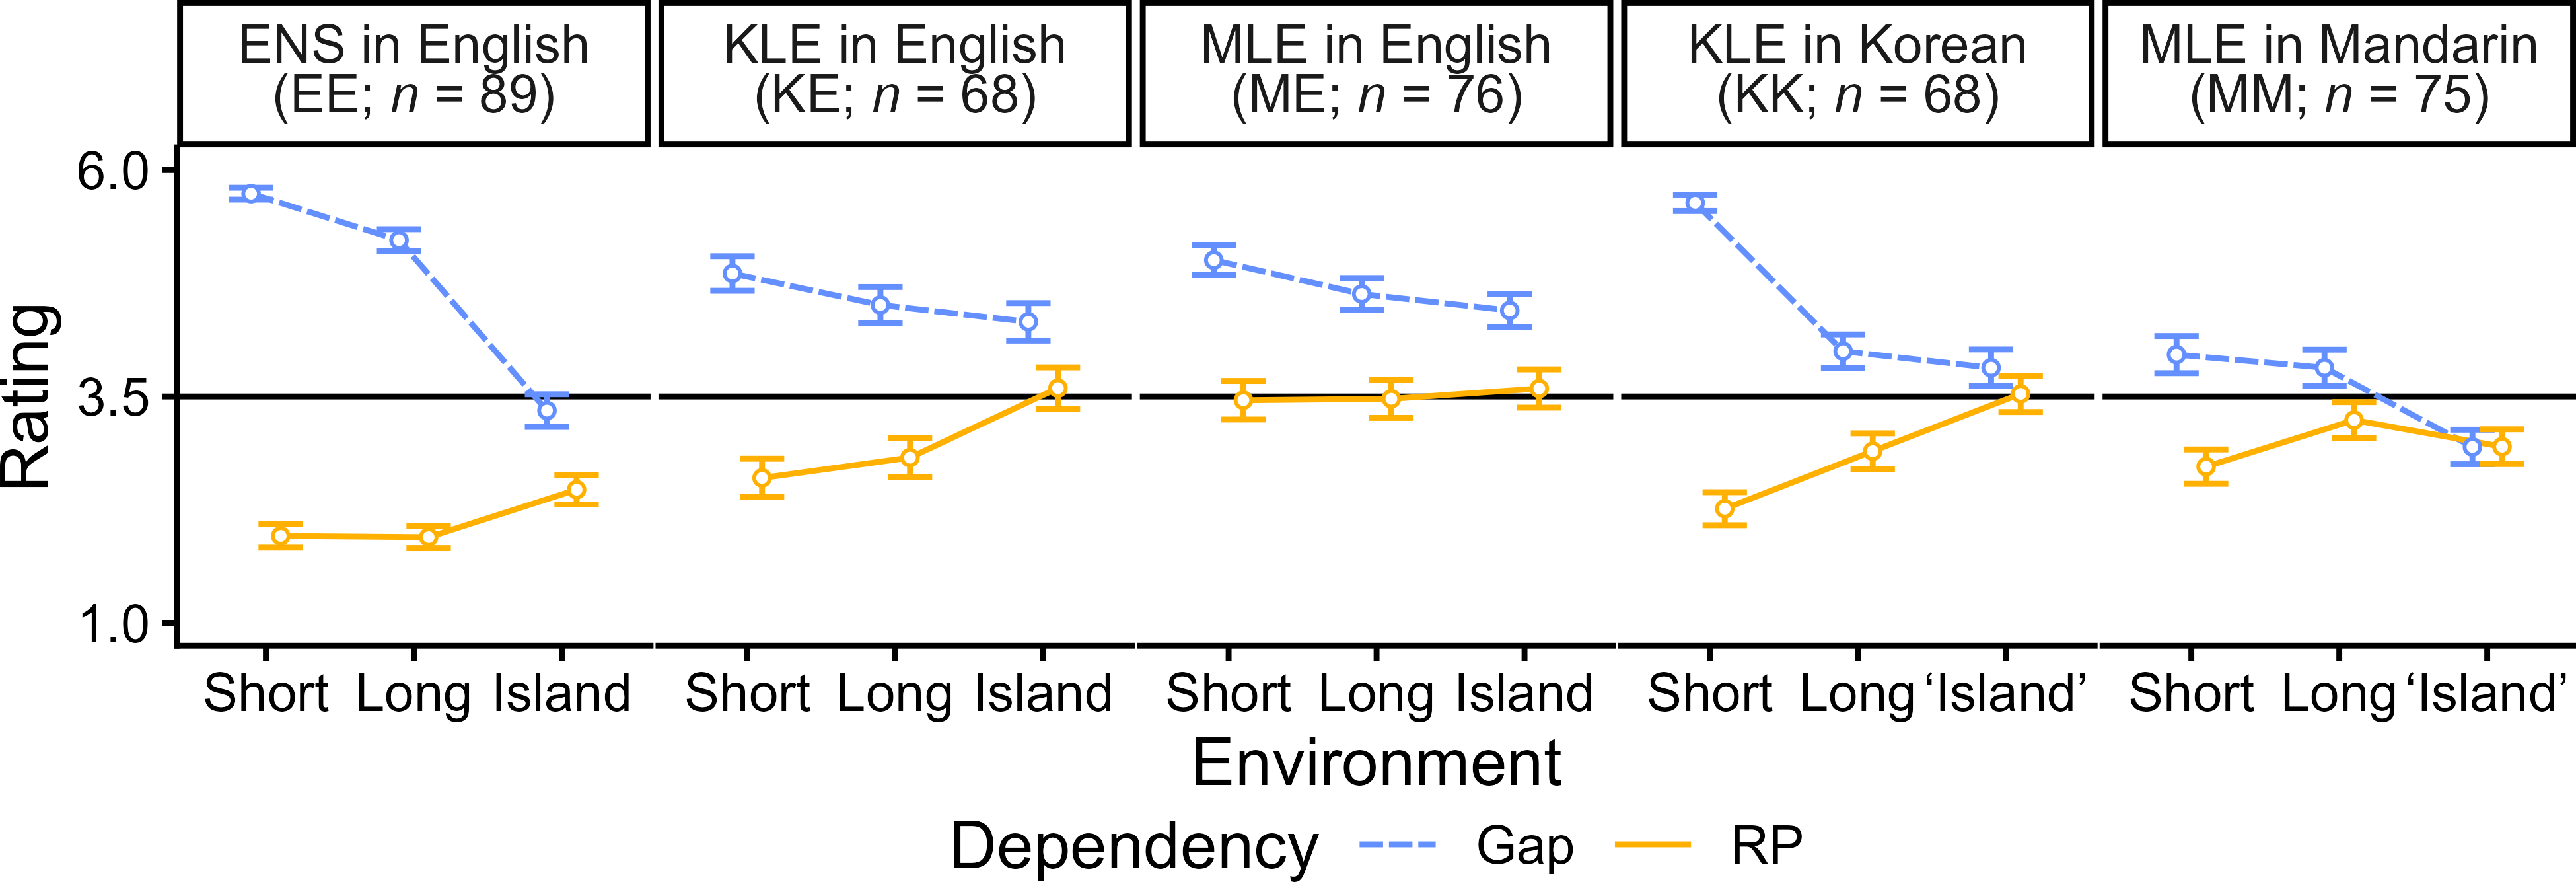
\includegraphics[width=\textwidth]{../analysis/plots/orc_ajt_rating.png}
\textit{Note}. Error bars are 95\% \textit{CI}s; the horizontal line marks the scale's midpoint.
\vspace{-12pt}
\end{figure}

\begin{figure}
\caption{Mean ratings for critical trials in the SRC acceptability judgment task} \label{fig:ajt-rating-src}
\raggedright\setstretch{1}
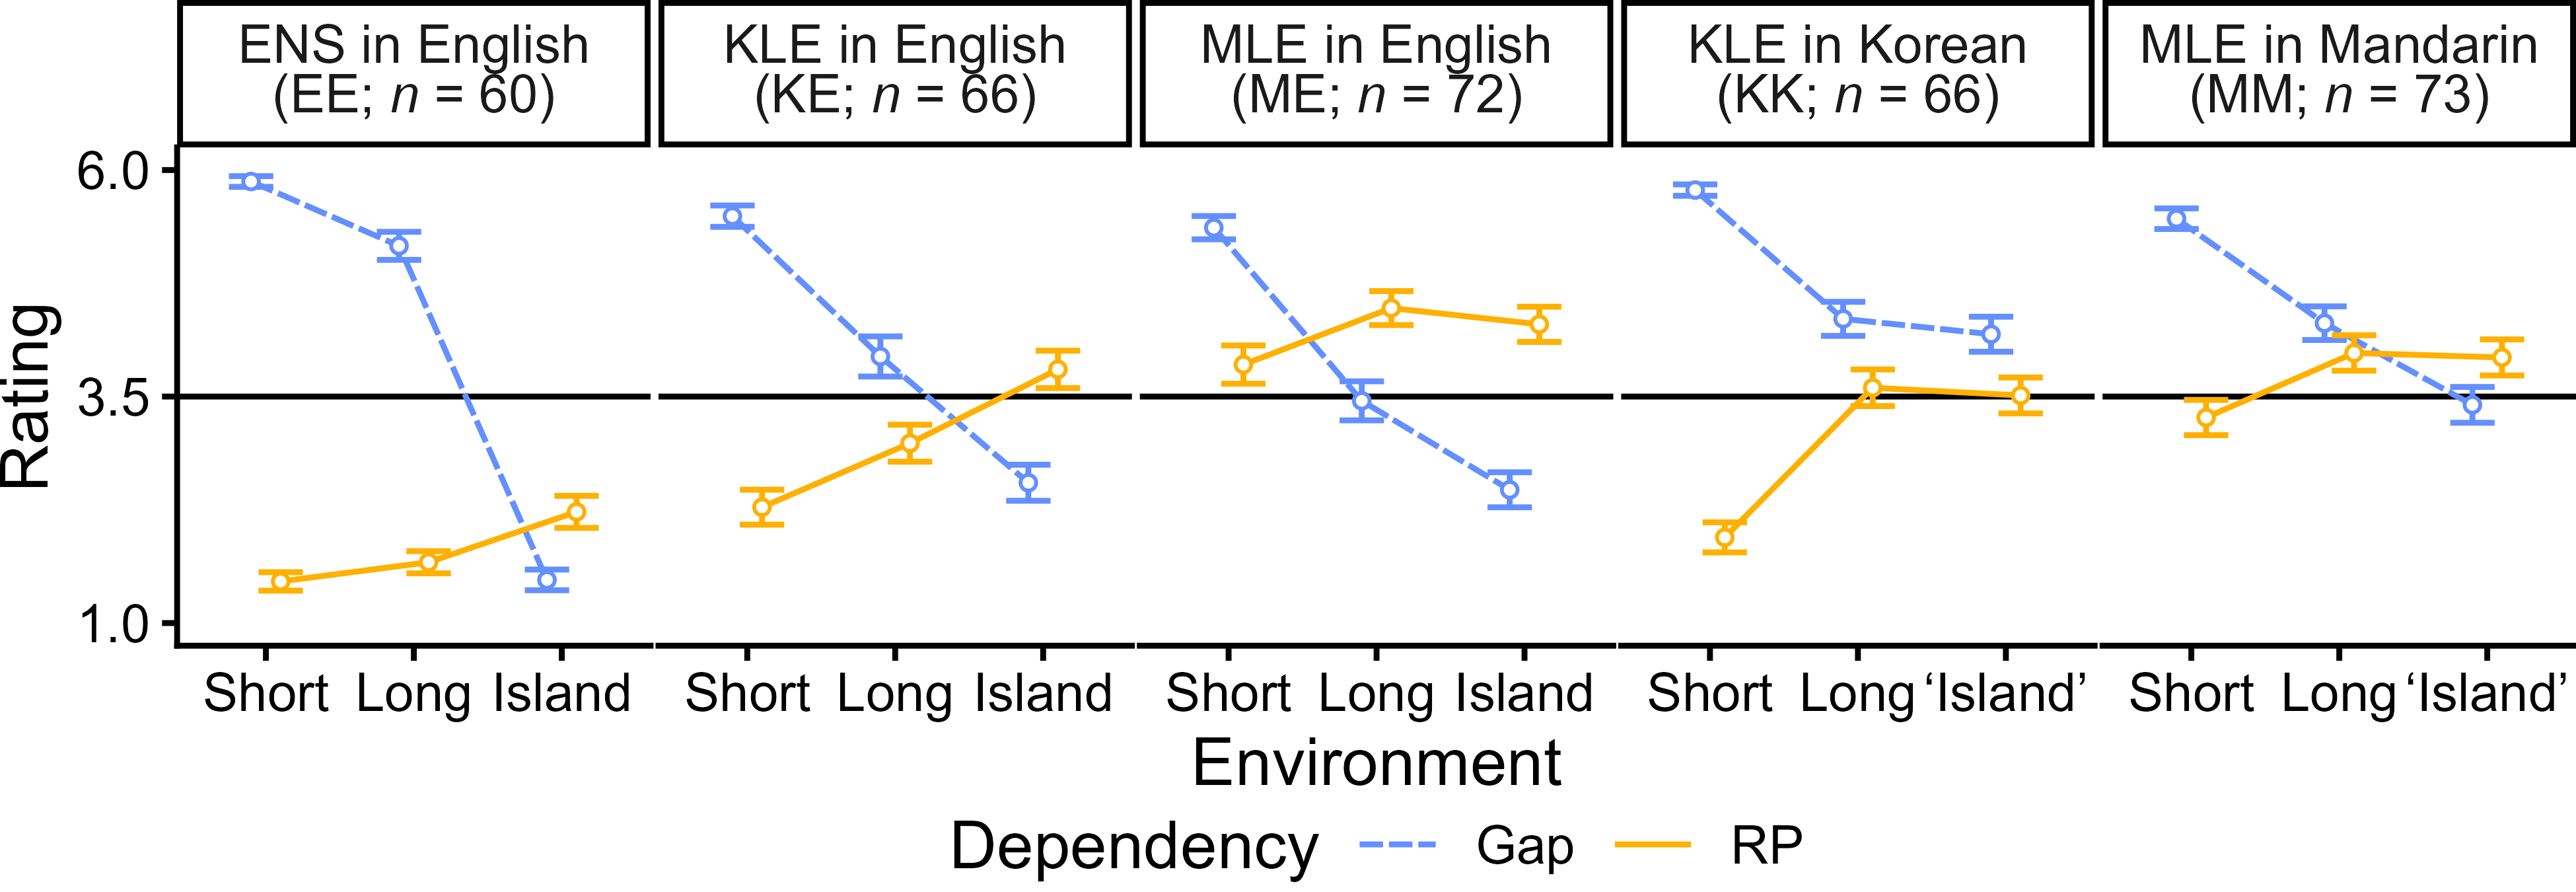
\includegraphics[width=\textwidth]{../analysis/plots/src_ajt_rating.png}
\textit{Note}. Error bars are 95\% \textit{CI}s; the horizontal line marks the scale's midpoint.
\vspace{-12pt}
\end{figure}

\noindent ENSs judged gaps to be highly acceptable in the Short and Long conditions, where they are grammatical in English. By contrast, they judged gaps to be highly unacceptable in the Island condition, where they are ungrammatical in English---at least in the SRC data. In the ORC data, the 95\% \textit{CI} for gap ratings in the Island condition straddled the midpoint of the rating scale, indicating that \textit{wh}-island ORCs are relatively weak islands. In RP trials, the ENS group's ratings were consistently on the bottom half of the scale, indicating that they considered RPs unacceptable. However, their mean RP ratings did increase subtly from the Short (easiest) condition to the Island (hardest) condition, which I~interpret as a sign of the processing facilitation conferred by resumption in difficult-to-parse RCs.

Compared to the ENS group, the KLE and MLE groups tended to give lower ratings to English gaps in the Long condition (which are grammatical, though more difficult to process than gaps in the Short condition) and higher ratings to English gaps in the Island condition (which are ungrammatical). For English RPs, KLEs and MLEs gave higher ratings than ENSs across all three environments; they were highest among MLEs, hugging the midpoint of the scale in the ORC dataset and extending into the upper half of the scale in the SRC dataset.

When tested in their L1, KLEs and MLEs gave ratings that were largely similar to the ones they gave in English. However, there were two notable points of difference: First, KLEs and MLEs gave higher ratings to SRC `Island' gaps in their L1 than in English, with KLEs consistently accepting Korean gaps but not English gaps in that condition. As a reminder, I expected that there would be high rates of gap acceptance in the KK and MM `Island' conditions, just like in the Long conditions (see~Section~\ref{gap-lw} and \ref{acq-slw-pathway}). Second, MLEs tended to rate RPs somewhat lower in Mandarin than they did in English; in the ORC data, for instance, the 95\% \textit{CI}s for their RP ratings straddled the midpoint of the scale across all three ME conditions but were restricted to the lower half of the scale for all three MM conditions. Overall, ratings for Korean RPs were somewhat higher than expected, though they never met the criteria for consistent acceptance (see~Section~\ref{ajt-analysis} above). By contrast, ratings for Mandarin RPs were somewhat lower than expected, especially in the ORC dataset (for discussion, see Section~\ref{dis-kozh}).

In filler trials (see Appendix~\ref{app-results-ajt}, Section~\ref{app-ajt-filler}), ratings were generally high for grammatical trials, with means and 95\% \textit{CI}s above the midpoint of 3.5 in all \textsc{pairing} × \textsc{type} combinations. Ratings tended to be very low for ungrammatical trials, with means and \textit{CI}s below the midpoint in almost all \textsc{pairing} × \textsc{type} combinations; the one exception was the F2U fillers, which (as~predicted) L2ers tended to rate as acceptable.

I~further examined the patterns in the critical-trial data by fitting the ratings from the ORC and SRC datasets to separate cumulative link mixed models. 

The ORC model (model formula: \textsc{rating \~{} dependency * environment * pairing + (1 + dependency + environment | participant) + (1 + dependency + environment + pairing | item)}---see Appendix~\ref{app-results-ajt}, Table~\ref{tblr:app-orc-ajt-rating-model} for details) turned up significant effects for (a)~\textsc{dependency}, with ratings tending to be higher for gaps than for RPs ($\hat{\beta}$~=~−2.28, \textit{SE}~=~0.15, $p$~<~.001), and (b)~\textsc{environment}, with ratings tending to be lower in the Long and Island/`Island' conditions than in the Short condition (Long~−~Short: $\hat{\beta}$~=~−0.33, \textit{SE}~=~0.07, $p$~<~.001; Island/`Island'~−~Short: $\hat{\beta}$~=~−0.54, \textit{SE}~=~0.10, $p$~<~.001). In English, there were also marginal-to-significant effects for \textsc{pairing}, with KLEs and MLEs tending to give higher ratings than ENSs (KE~−~EE: $\hat{\beta}$~=~0.37, \textit{SE}~=~0.21, $p$~=~.069; ME~−~EE: $\hat{\beta}$~=~0.69, \textit{SE}~=~0.20, $p$~=~.001). Most of the two-way and three-way interactions came out as significant (p~<~.05) as well. Crucially, pairwise comparisons revealed that in English, ratings were significantly higher for gaps than for RPs in all \textsc{environment} × \textsc{pairing} combinations (all $p$s~<~.05). Taken together with the generally low mean ratings for RPs, these results suggest that no group (as a group) regarded resumption as an acceptable means of English ORC formation in any environment tested. In the Korean and Mandarin AJTs, the group results were similar to those in English in that the gap-over-RP preference was significant in the Short and Long conditions (all $p$s~<~.05); however, unlike in their English AJT results, for neither KLEs in Korean nor MLEs in Mandarin did the contrast approach significance in their L1 `Island' condition (both $p$s~>~.10).

The SRC model (model formula: \textsc{rating \~{} dependency * environment * pairing + (1 + dependency + environment | participant) + (1 + dependency + environment + pairing | item)}---see Appendix~\ref{app-results-ajt}, Table~\ref{tblr:app-src-ajt-rating-model} for details) found significant effects for (a)~\textsc{dependency}, with RPs having lower ratings than gaps ($\hat{\beta}$~=~−1.59, \textit{SE}~=~0.10, $p$~<~.001), (b)~\textsc{environment}, with the Long condition and the Island/`Island'-condition both having lower ratings than the Short condition (Long~−~Short: $\hat{\beta}$~=~−0.64, \textit{SE}~=~0.10, $p$~<~.001; Island/`Island'~−~Short: $\hat{\beta}$~=~−1.48, \textit{SE}~=~0.12, $p$~<~.001), and (c)~\textsc{pairing}, with KLEs and MLEs, in English and their L1, tending to give higher ratings than ENSs (KE~−~EE: $\hat{\beta}$~=~0.60, \textit{SE}~=~0.21, $p$~=~.005; ME~−~EE: $\hat{\beta}$~=~1.24, \textit{SE}~=~0.21, $p$~<~.001; KK~−~EE: $\hat{\beta}$~=~1.10, \textit{SE}~=~0.21, $p$~<~.001; MM~−~EE: $\hat{\beta}$~=~1.33, \textit{SE}~=~0.21, $p$~<~.001). Most of the two-way and three-way interactions also came out as significant ($p$~<~.05). In the pairwise comparisons, the [RP~−~gap] contrast was found to be significant in all \textsc{pairing} × \textsc{environment} combinations in English: Gaps were rated significantly higher than RPs for all groups in the Short condition (ENS: $\hat{\beta}$~=~−7.03, \textit{SE}~=~0.31, $p$~<~.001; KLE: $\hat{\beta}$~=~−4.41, \textit{SE}~=~0.23, $p$~<~.001; MLE: $\hat{\beta}$~=~−2.15, \textit{SE}~=~0.22, $p$~<~.001) and for ENSs and KLEs in the Long condition (ENS: $\hat{\beta}$~=~−4.54, \textit{SE}~=~0.25, $p$~<~.001; KLE: $\hat{\beta}$~=~−1.28, \textit{SE}~=~0.22, $p$~<~.001); by contrast, RPs were rated significantly higher than gaps for all groups in the Island condition (ENS: $\hat{\beta}$~=~1.10, \textit{SE}~=~0.25, $p$~<~.001; KLE: $\hat{\beta}$~=~1.39, \textit{SE}~=~0.22, $p$~<~.001; MLE: $\hat{\beta}$~=~2.21, \textit{SE}~=~0.21, $p$~<~.001) and for MLEs also in the Long condition ($\hat{\beta}$~=~1.17, \textit{SE}~=~0.21, $p$~<~.001). For KLEs in the Korean AJT, RP ratings were significantly lower than gap ratings across all three environments (Short: $\hat{\beta}$~=~−5.66, \textit{SE}~=~0.26, $p$~<~.001; Long: $\hat{\beta}$~=~−0.90, \textit{SE}~=~0.21, $p$~<~.001; `Island': $\hat{\beta}$~=~−0.78, \textit{SE}~=~0.21, $p$~=~.003). By contrast, for MLEs in the Mandarin AJT, the [RP~−~gap] contrast was found to be significant in only the Short condition, where RPs were rated lower than gaps ($\hat{\beta}$~=~−3.00, \textit{SE}~=~0.21, $p$~<~.001); they also exhibited a marginally significant gap-over-RP preference in the Long condition ($\hat{\beta}$~=~−0.55, \textit{SE}~=~0.20, $p$~=~.080) and a marginally significant RP-over-gap preference in the `Island' condition ($\hat{\beta}$~=~0.54, \textit{SE}~=~0.20, $p$~=~.083).

To summarize, RP ratings tended to increase at least slightly down the SLW hierarchy for all levels of \textsc{pairing}. For ENSs, the mean RP ratings remained low across environments, only overtaking the mean gap rating in the SRC Island condition, where (a)~gaps are ungrammatical in English and (b)~both conditions were consistently rated on the lower half of the rating scale. The fact that RP ratings overtook gap ratings in the SRC Island condition but not the ORC Island condition attests to the increased strength of SRC islands relative to ORC islands, i.e., gaps in \textit{wh}-island SRCs have particularly low acceptability (\cite{han.etal2012}, p.~157; \cite{mcdaniel.cowart1999}, p.~B21; \cite{morgan.wagers2018}, p.~867).\footnotemark{} Compared to the ENS group, the KLE and MLE groups tended to have lower ratings for English gaps and higher ratings for English RPs. The fact that the two L2 groups both consistently rated English RPs on the upper half of the rating scale in one or more SRC environments---in many cases preferring them over English gaps by a significant margin---suggests that the interlanguage English grammars of some of these KLEs and MLEs may license RPs in certain types of difficult-to-process RCs. Furthermore, the fact that ratings for gaps tended to be higher in the KK and MM pairings than in the EE pairing suggests that at least some cases of English RP acceptance among KLEs and MLEs may be traceable to L1 transfer.

\footnotetext{As mentioned in Section~\ref{res-wellformedness}, \textcite{mcdaniel.cowart1999} suggest that \textit{wh}-island SRCs are worse than \textit{wh}-island ORCs because they violate an additional syntactic constraint: the Empty Category Principle (Chomsky, 1981).}

%========================================================%
\section{L2 proficiency effects for by-group rating patterns}\label{ajt-rating-proficiency}
%========================================================%

Now let us consider the relation between English proficiency and L2ers' by-group rating patterns in the English AJT. Figures \ref{fig:ajt-rating-proficiency-orc} and \ref{fig:ajt-rating-proficiency-src} show the relationship between L2ers' scaled English proficiency scores and their mean ratings in, respectively, the ORC data and the SRC data. One MLE in the SRC dataset had to be excluded from this analysis because of a missing proficiency score. There was an overwhelming tendency for a gap-over-RP preference in ratings to emerge as proficiency scores get higher. 

\begin{figure}
\caption{Relationship between L2 proficiency and ratings in the English ORC acceptability judgment task} \label{fig:ajt-rating-proficiency-orc}
\raggedright\setstretch{1}
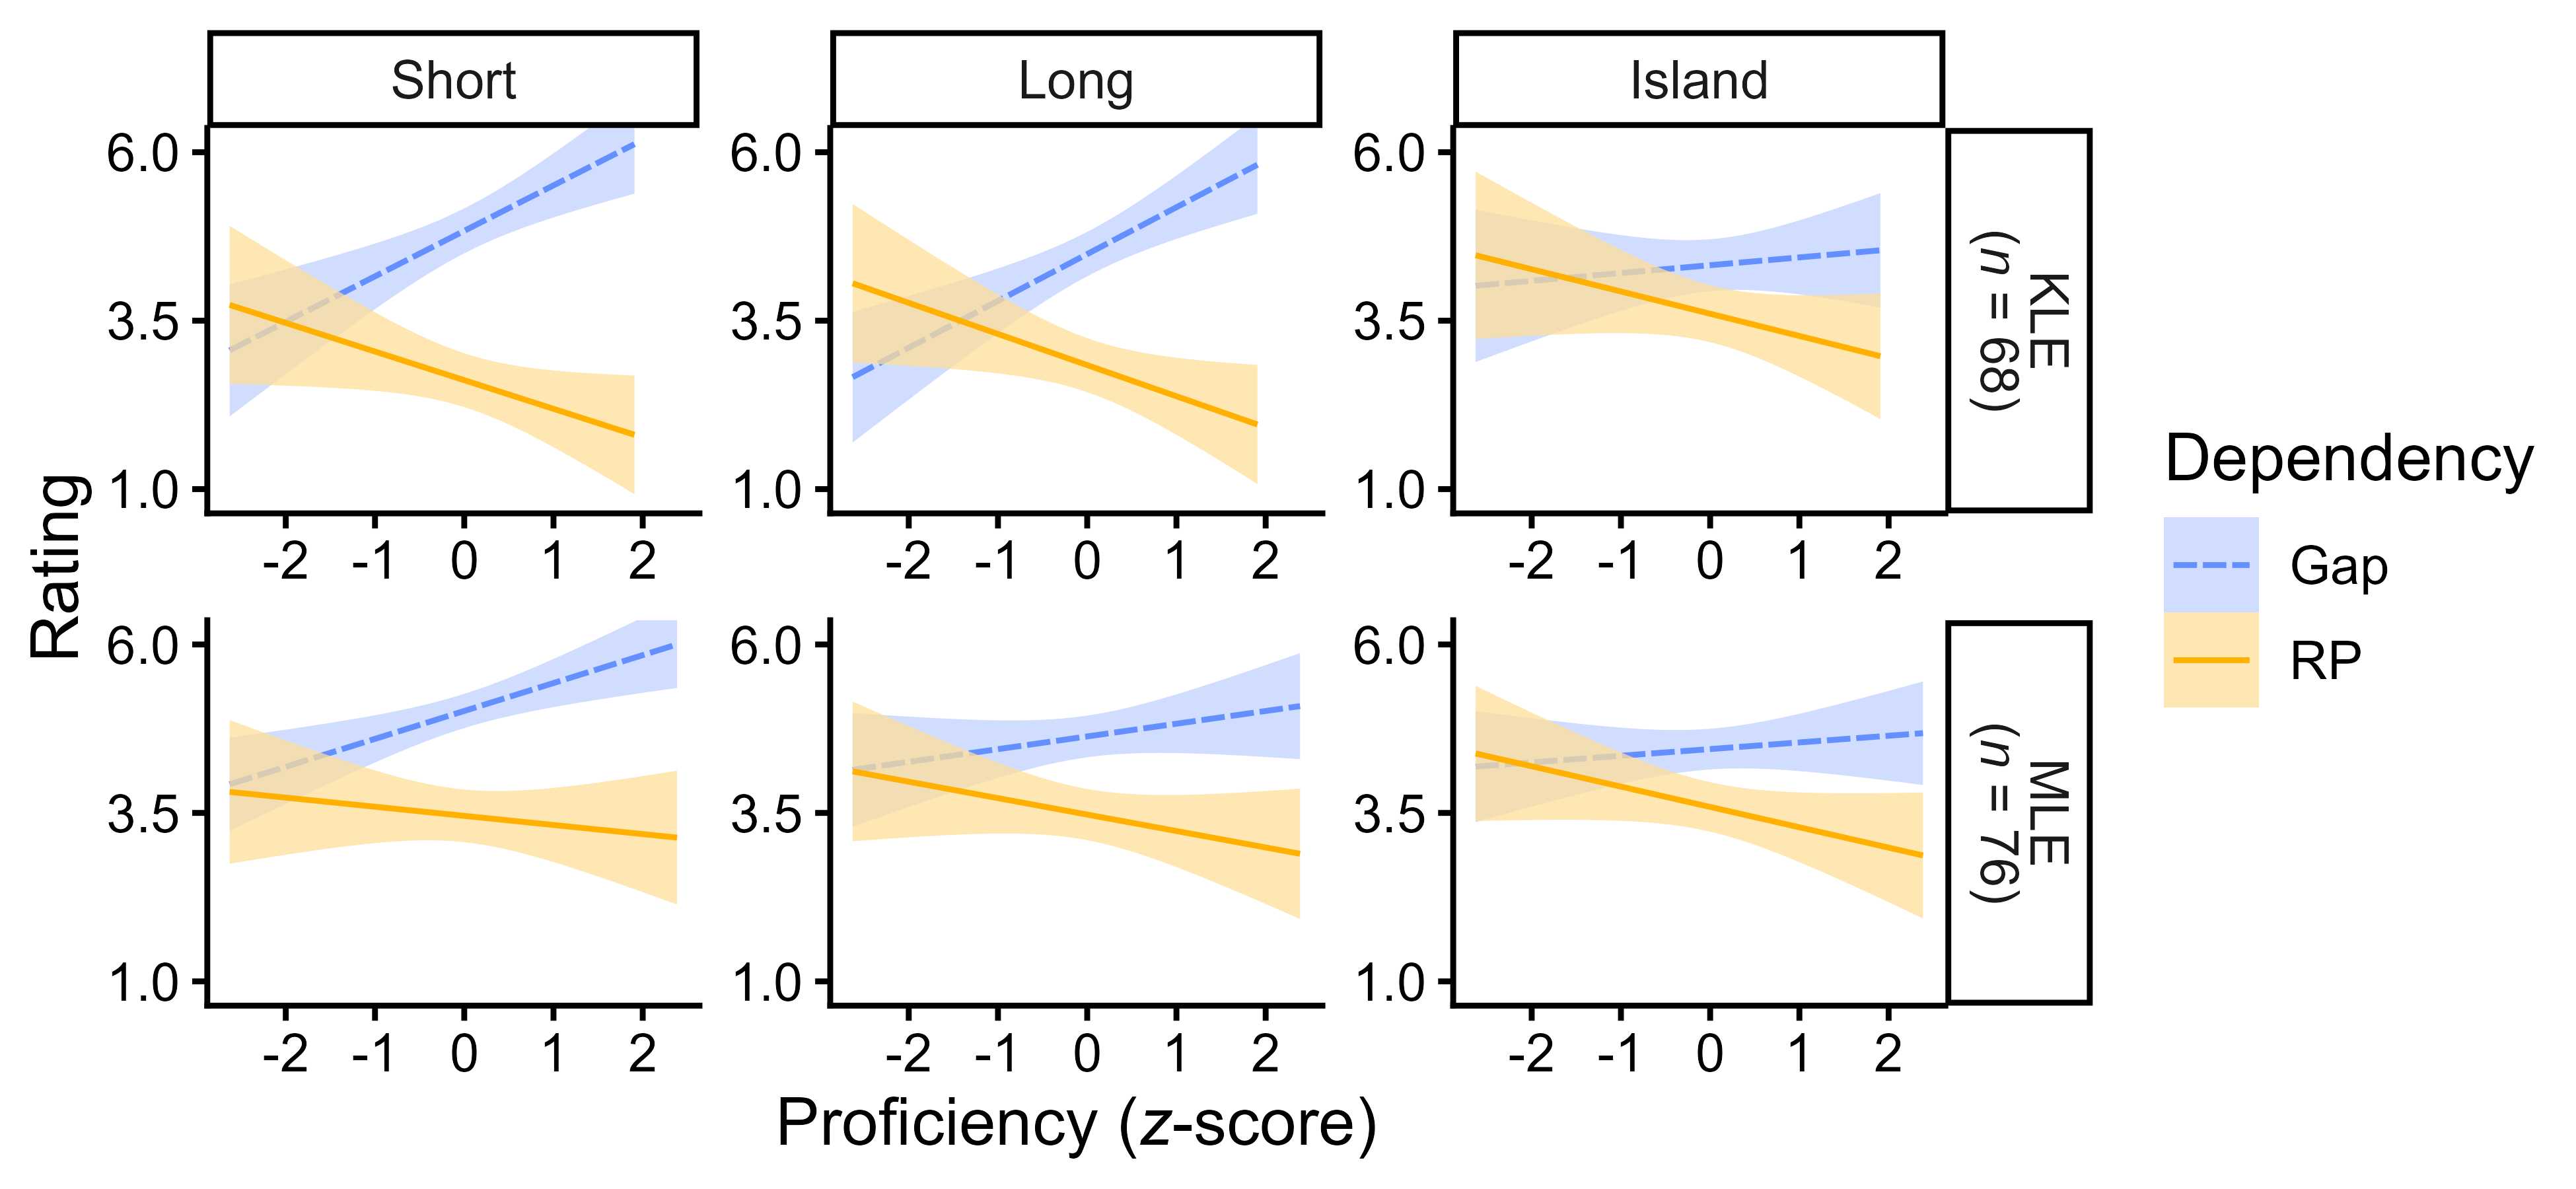
\includegraphics[width=\textwidth]{../analysis/plots/orc_ajt_rating_proficiency.png}
\textit{Note}. Shading indicates 95\% \textit{CI}s.
\vspace{-12pt}
\end{figure}

\begin{figure}
\caption{Relationship between L2 proficiency and ratings in the English SRC acceptability judgment task} \label{fig:ajt-rating-proficiency-src}
\raggedright\setstretch{1}
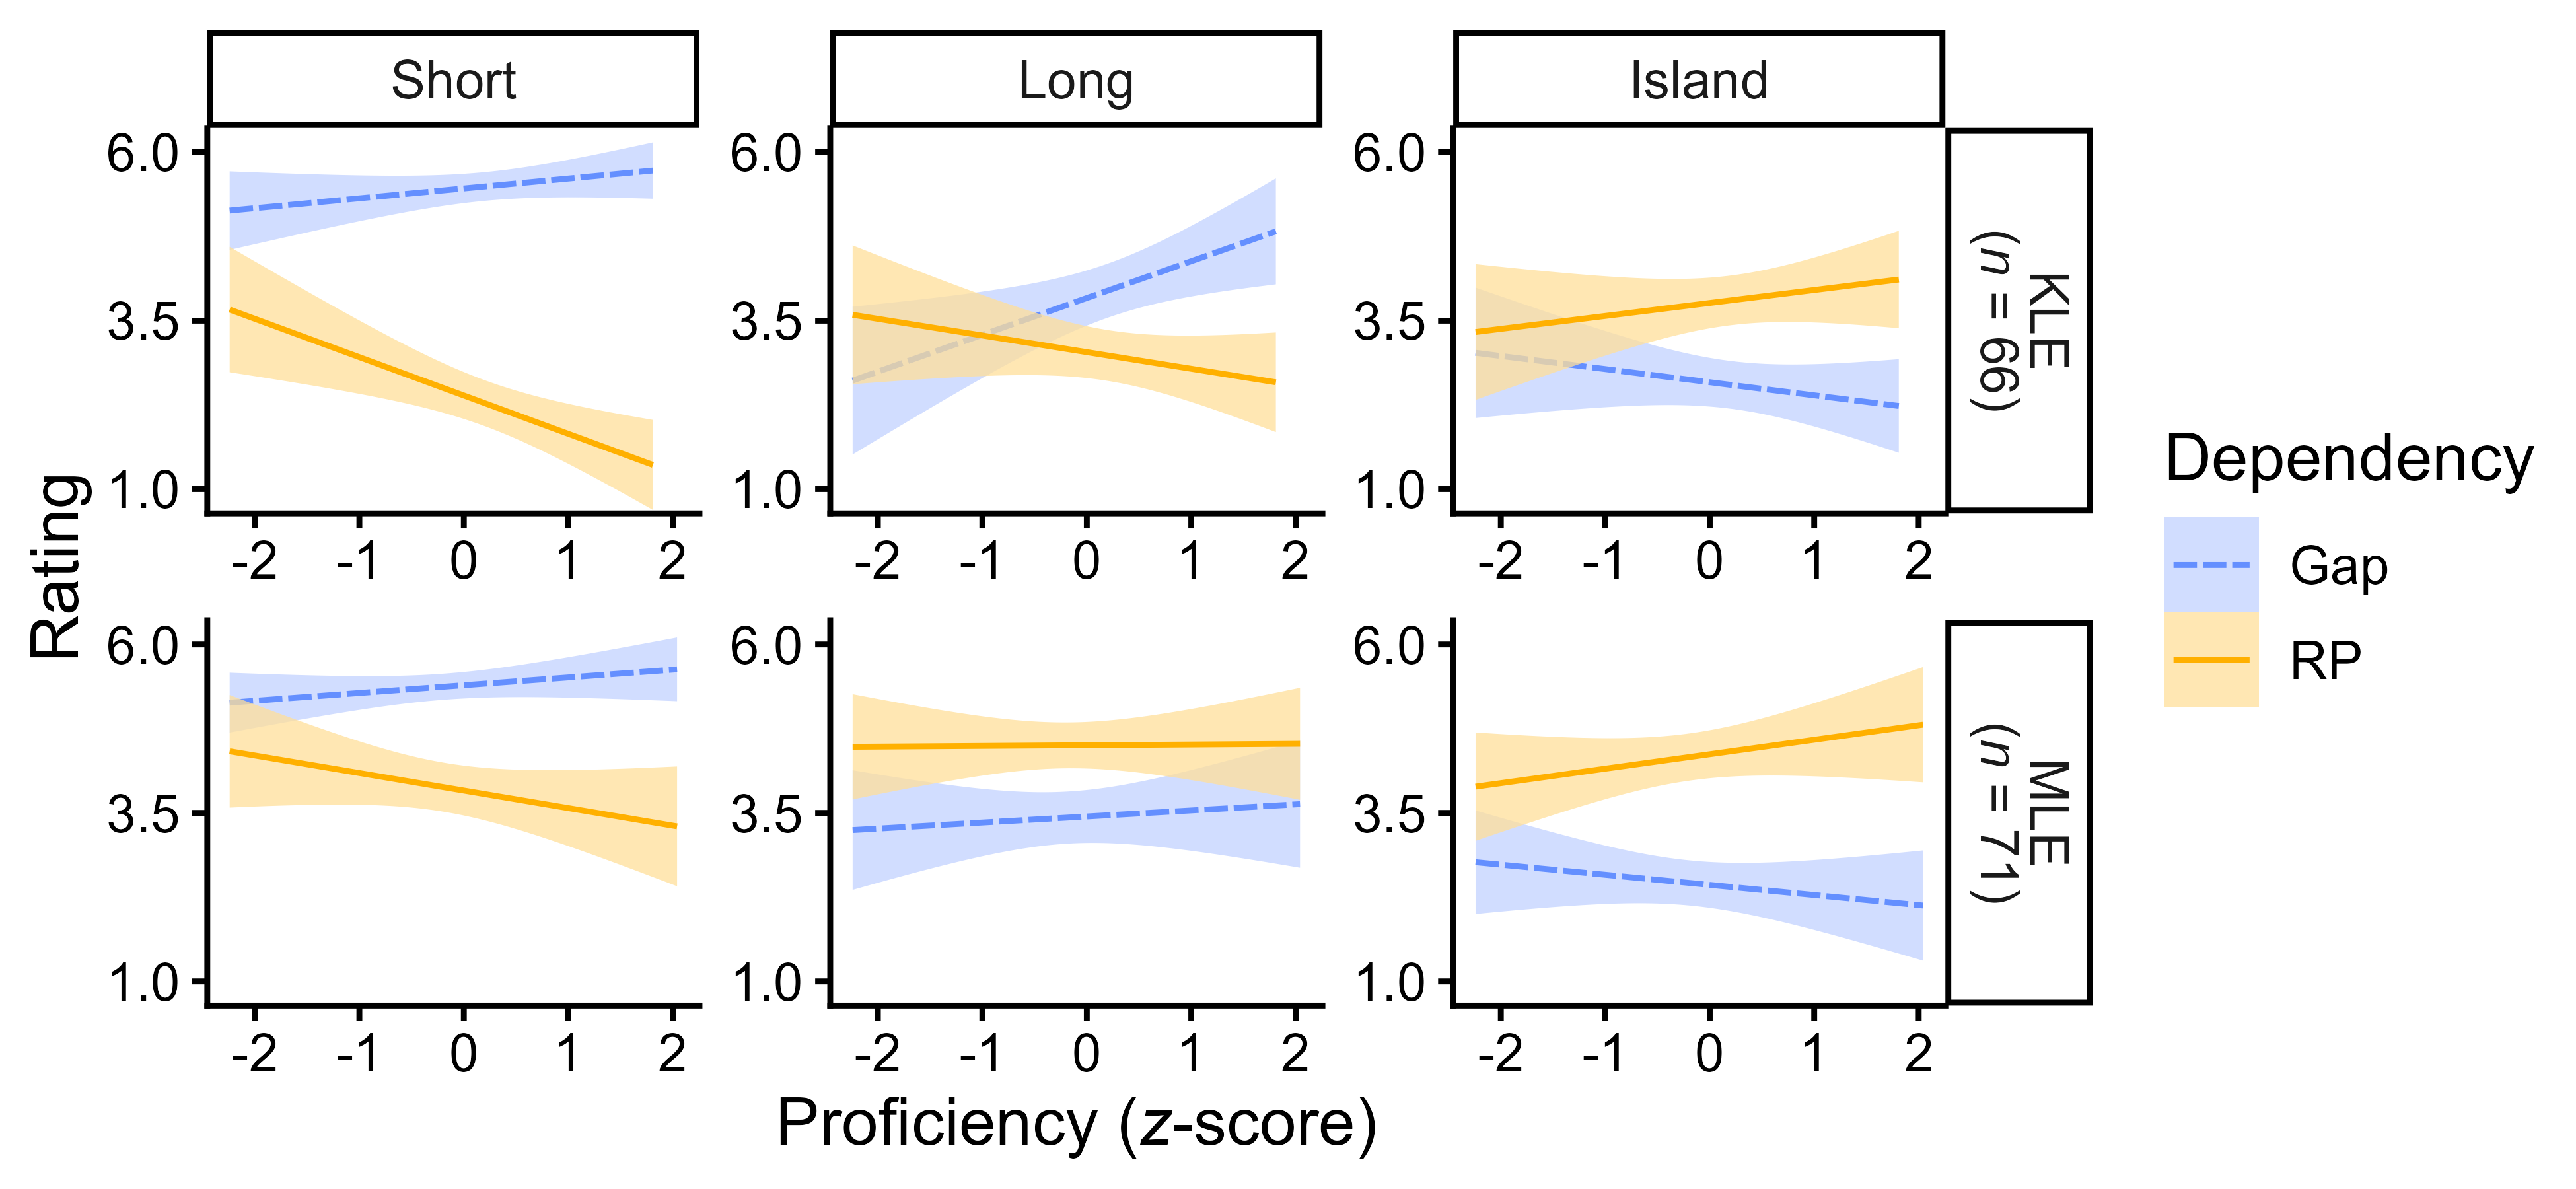
\includegraphics[width=\textwidth]{../analysis/plots/src_ajt_rating_proficiency.png}
\textit{Note}. Shading indicates 95\% \textit{CI}s.
\vspace{-12pt}
\end{figure}

\noindent The effect appears to be strongest towards the top of the SLW hierarchy, where processing should be easiest. The only exceptions to this pattern were (a)~the SRC Long condition for MLEs only and (b)~the SRC Island condition for both KLEs and MLEs. That RPs should be preferred over gaps across the proficiency spectrum in the SRC Island condition is to be expected if it is correct to think that in English (a)~\textit{wh}-island SRCs are stronger islands than \textit{wh}-island ORCs (see~fn.~3) and (b)~\textit{wh}-island SRCs place even more strain on the processor than \textit{wh}-island ORCs (see~Section~\ref{gap-wi}).

I~continued to probe for L2 proficiency effects in the rating data by refitting the ORC and SRC models with the data filtered to the KE and ME pairings and with \textsc{proficiency} added as a continuous fixed effect. 

The ORC model (model formula: \textsc{rating \~{} dependency * environment * pairing * proficiency + (1 + dependency * environment | participant) + (0 + dependency * environment | item)}---see Appendix~\ref{app-results-ajt}, Table~\ref{tblr:app-orc-ajt-rating-proficiency-model} for details) yielded no main effect for \textsc{proficiency} ($p$~=~.217). However, there was a significant \textsc{dependency} × \textsc{proficiency} interaction ($\hat{\beta}$~=~−1.41, \textit{SE}~=~0.36, $p$~<~.001), indicating that the gap-over-RP preference in ratings became more pronounced as proficiency scores rose. Several of the other interactions involving \textsc{proficiency} also reached significance, and post-hoc tests revealed that the \textsc{dependency} × \textsc{proficiency} interaction was strongest for KLEs, reaching significance in the Short and Long conditions (Short: $\hat{\beta}$~=~−3.03, \textit{SE}~=~0.64, $p$~<~.001; Long: $\hat{\beta}$~=~−2.39, \textit{SE}~=~0.56, $p$~<~.001).

As with the ORC model, the SRC model (model formula: \textsc{rating \~{} dependency * environment * pairing * proficiency + (1 + dependency * environment | participant) + (1 + dependency * environment | item)}---see Appendix~\ref{app-results-ajt}, Table~\ref{tblr:app-src-ajt-rating-proficiency-model} for details) found no significant effect of \textsc{proficiency} ($p$~=~.664). However, several of the two-way and three-way interactions involving \textsc{proficiency} did come out as significant, and pairwise comparisons revealed that the \textsc{dependency} × \textsc{proficiency} interaction was statistically meaningful for KLEs in both the Short condition ($\hat{\beta}$~=~−1.90, \textit{SE}~=~0.50, $p$~=~.001) and the Long condition ($\hat{\beta}$~=~−1.33, \textit{SE}~=~0.49, $p$~=~.038), with the gap-over-RP preference becoming stronger as proficiency increased.

Overall, these results indicate that as gains are made in English proficiency, L2ers become more sensitive to the fact that English allows gapping but not resumption in RCs. This sensitivity appears to develop faster towards the top of the SLW hierarchy, where processing is expected to be easiest.

%========================================================%
\section{By-participant rating patterns}\label{ajt-individual}
%========================================================%

Next, let us consider RQ2, which asks how individual response patterns compared to the group means in the rating data. I~took the fact that several of the by-group means for RPs were at or near the middle of the rating scale as a hint that there may have been large differences in performance among individual participants. To explore this possibility, I~sorted participants into categories based on the consistency/inconsistency of their rating patterns. Those who gave `acceptable' ratings (4, 5, or 6) on at least four out of five RP trials in a given condition were labeled `RP acceptors,' and those who gave `unacceptable' ratings (1, 2, or 3) on at least four out of five RP trials in a given condition were labeled `RP rejectors.' All other participants were categorized as `inconsistent raters.'

Figures~\ref{fig:ajt-acceptor-orc} and \ref{fig:ajt-acceptor-src} show the percentages of participants who were categorized as RP acceptors, RP rejectors, and inconsistent raters in, respectively, the ORC data and the SRC data. Although the numbers of RP acceptors and inconsistent raters were in some cases very low, there was at least one RP acceptor, one RP rejector, and one inconsistent rater for each \textsc{environment} × \textsc{pairing} combination in the ORC dataset as well as in the SRC dataset. 

\begin{figure}
\caption{Percentage of RP acceptors, RP rejectors, and inconsistent raters by environment in the ORC acceptability judgment tasks} \label{fig:ajt-acceptor-orc}
\raggedright\setstretch{1}
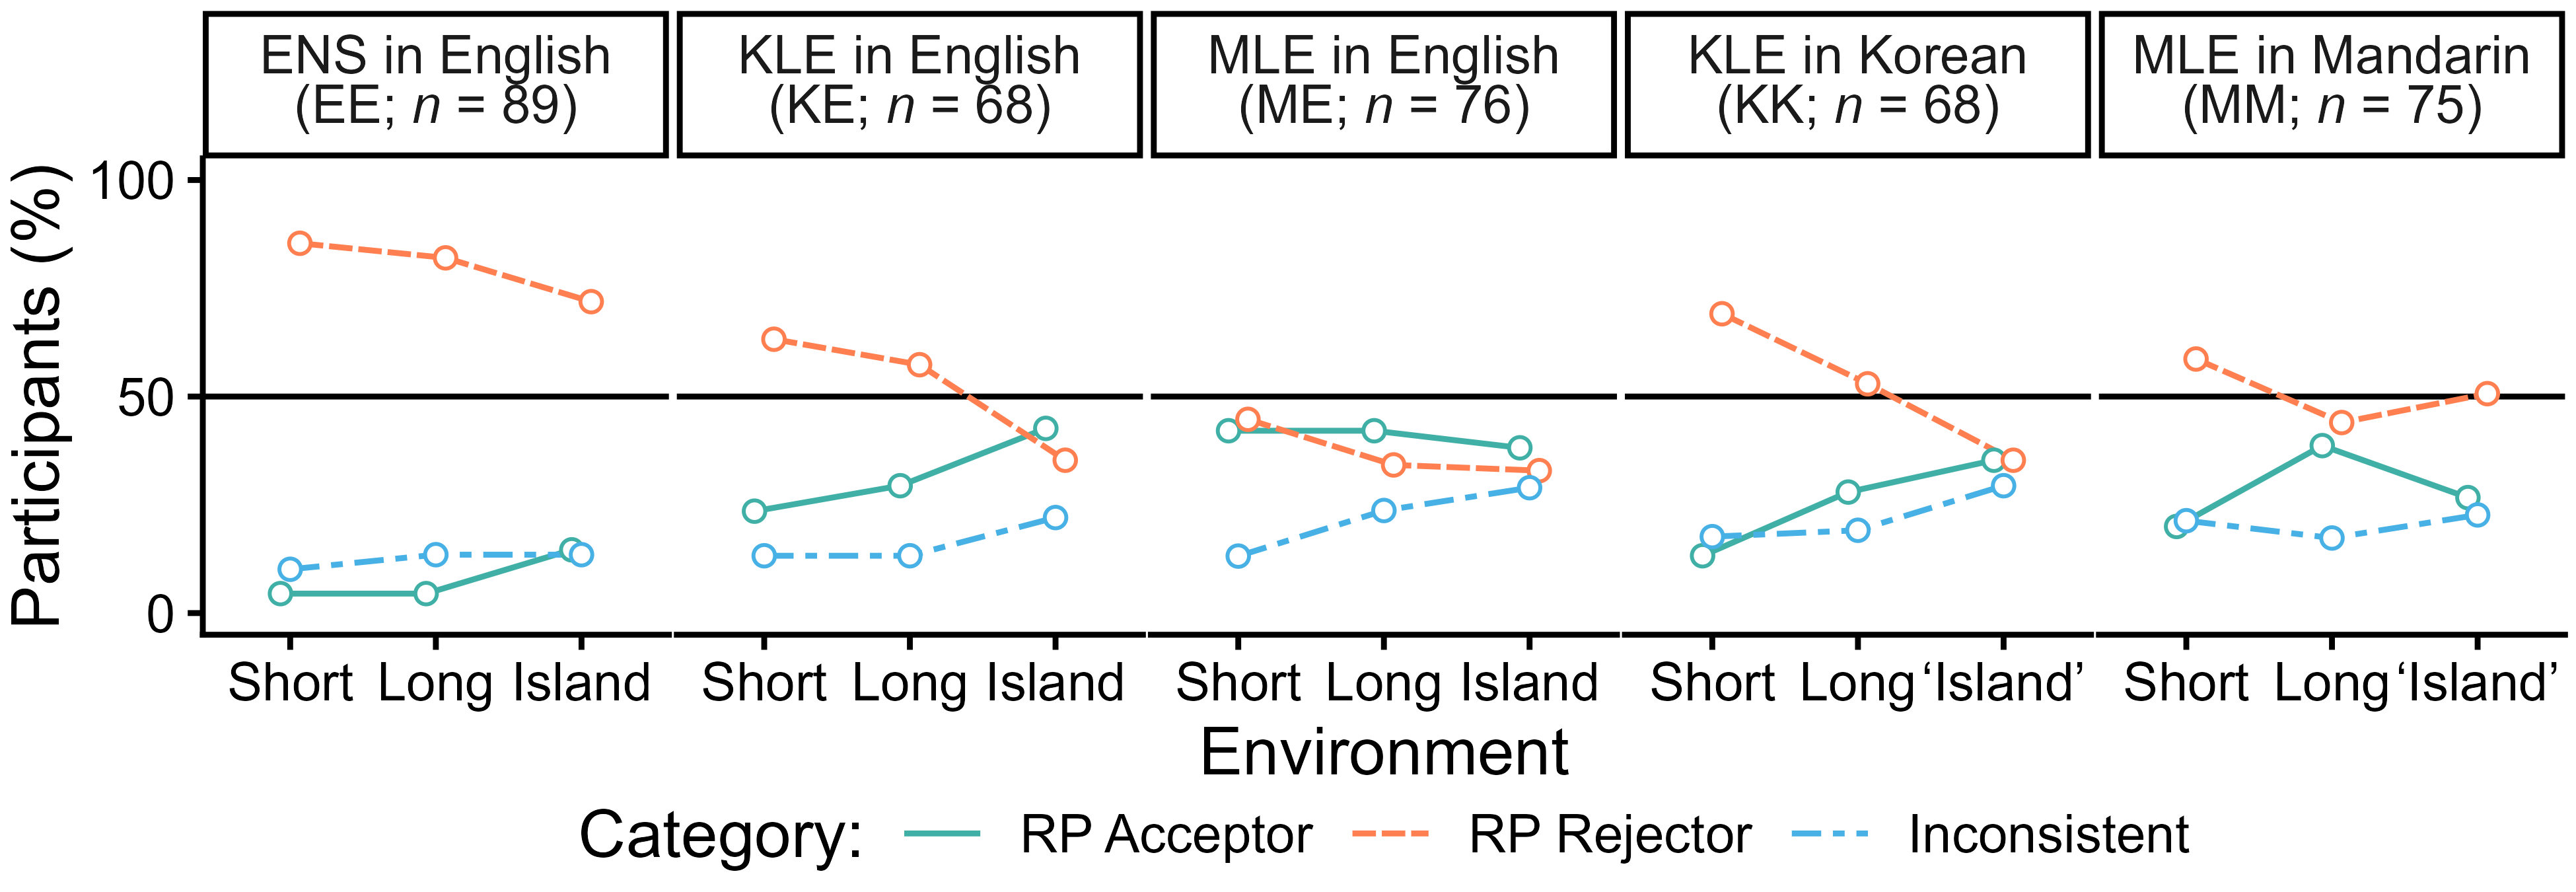
\includegraphics[width=\textwidth]{../analysis/plots/orc_ajt_acceptor.png}
\vspace{-24pt}
\end{figure}

\begin{figure}
\caption{Percentage of RP acceptors, RP rejectors, and inconsistent raters by environment in the SRC acceptability judgment tasks} \label{fig:ajt-acceptor-src}
\raggedright\setstretch{1}
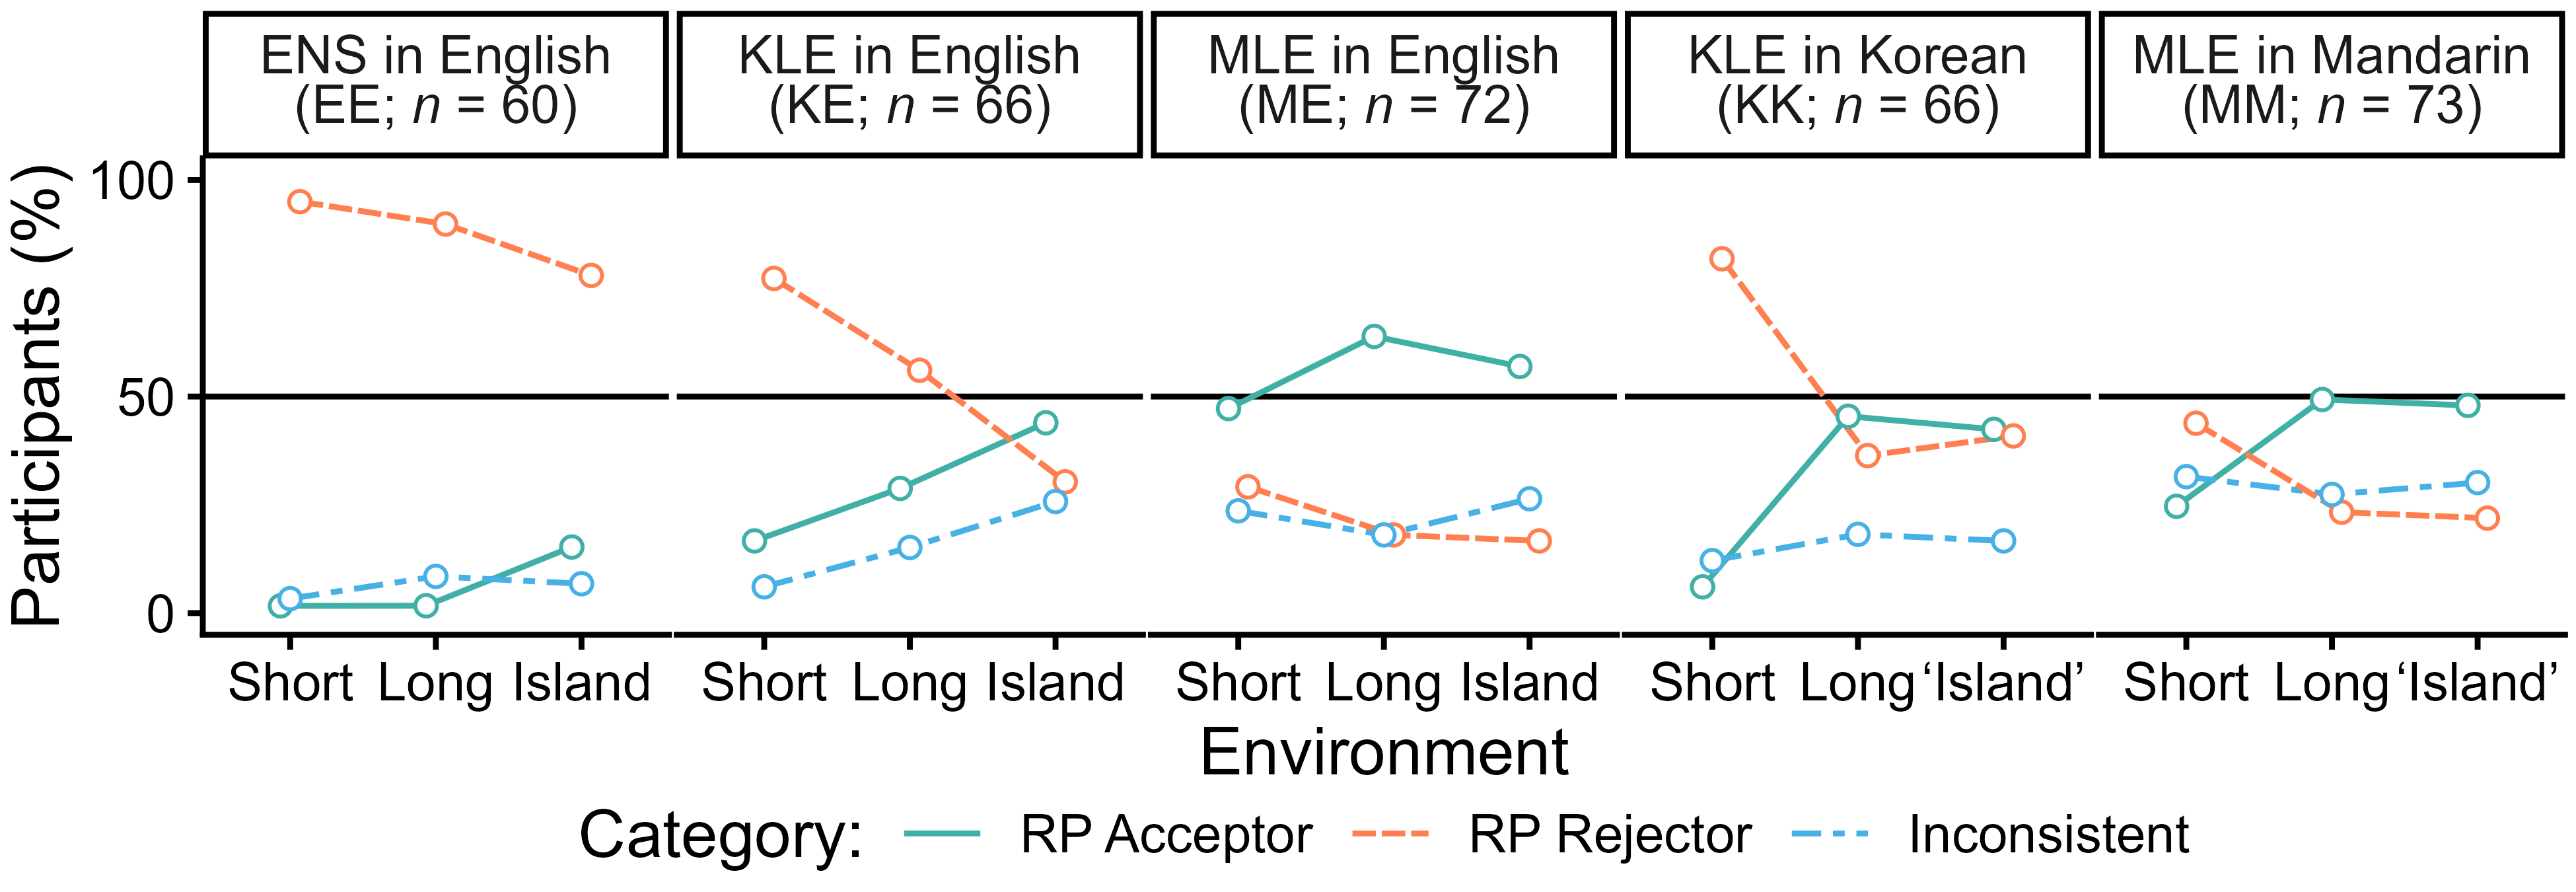
\includegraphics[width=\textwidth]{../analysis/plots/src_ajt_acceptor.png}
\vspace{-24pt}
\end{figure}

\noindent Despite the presence of some inconsistent raters, the majority of participants either consistently accepted or consistently rejected RPs in any given condition. The proportion of RP acceptors tended to increase from the Short condition to the Long and/or Island/`Island' conditions, whereas the opposite pattern was observed for RP rejectors. For ENSs, rates of RP rejection were high across the three environments, and only a small number consistently accepted RPs in any environment. The proportions of RP acceptors were decidedly higher for all other levels of \textsc{pairing}. Among KLEs, RP acceptors surpassed RP rejectors in the KE Island condition and were about on par with RP rejectors in the KK `Island' condition. A similar pattern was observed among MLEs in the Mandarin AJT, at least in the SRC dataset, where RP acceptors outnumbered RP rejectors in both the Long and `Island' conditions. RP acceptors were most common for MLEs in the SRC English AJT, ranging roughly from half to roughly two-thirds of participants across the three environments. There was thus a fairly large number of KLEs and MLEs who consistently accepted RPs when tested in English and/or their native language.

To further examine how rates of RP acceptance varied across levels of \textsc{environment} and \textsc{pairing}, I~fit participants' binary [\textsc{±acceptor}] scores to separate mixed-effects logistic regression models for the ORC and SRC datasets. 

The ORC model (model formula: \textsc{acceptor \~{} environment * pairing + (1 | participant)}---see Appendix~\ref{app-results-ajt}, Table~\ref{tblr:app-orc-ajt-acceptor-model} for details) yielded significant effects for (a)~\textsc{environment}, with the Long and Island/`Island' conditions having higher RP acceptance than the Short condition (Long~−~Short: $\hat{\beta}$~=~0.66, \textit{SE}~=~0.26, $p$~=~.010; Island/`Island'~−~Short: $\hat{\beta}$~=~1.06, \textit{SE}~=~0.24, $p$~<~.001), and (b)~\textsc{pairing}, with KE, ME, KK, and MM all having higher RP acceptance than EE (KE~−~EE: $\hat{\beta}$~=~2.83, \textit{SE}~=~0.54, $p$~<~.001; ME~−~EE: 3.49, \textit{SE}~=~0.54, $p$~<~.001; KK~−~EE: $\hat{\beta}$~=~2.32, \textit{SE}~=~0.54, $p$~<~.001; MM~−~EE: $\hat{\beta}$~=~2.54, \textit{SE}~=~0.54, $p$~<~.001). One of the two-way \textsc{environment} × \textsc{pairing} interactions also came out as significant ($p$~=~.014). Pairwise comparisons showed that the Short < Long contrast in RP acceptance was significant in the MM pairing ($\hat{\beta}$~=~1.51, \textit{SE}~=~0.48, $p$~=~.026) and that the Short < Island/`Island' contrast in RP acceptance was in the marginal-to-significant range in the KE pairing ($\hat{\beta}$~=~1.35, \textit{SE}~=~0.47, $p$~=~.055) and the KK pairing ($\hat{\beta}$~=~1.86, \textit{SE}~=~0.54, $p$~=~.007). For ENSs, RP acceptance was not found to increase significantly across conditions.

As with the ORC model, the SRC model (model formula: \textsc{acceptor \~{} environment * pairing + (1 | participant)}---see Appendix~\ref{app-results-ajt}, Table~\ref{tblr:app-src-ajt-acceptor-model} for details) found significant effects for (a)~\textsc{environment}, with the Long and Island/`Island' conditions having higher RP acceptance than the Short condition (Long~−~Short: $\hat{\beta}$~=~1.20, \textit{SE}~=~0.35, $p$~<~.001; Island/`Island'~−~Short: $\hat{\beta}$~=~1.74, \textit{SE}~=~0.29, $p$~<~.001), and (b)~\textsc{pairing}, with the KE, ME, KK, and MM pairings all having higher RP acceptance than the EE pairing (KE~−~EE: $\hat{\beta}$~=~2.59, \textit{SE}~=~0.57, $p$~<~.001; ME~−~EE: $\hat{\beta}$~=~4.00, \textit{SE}~=~0.57, $p$~<~.001; KK~−~EE: $\hat{\beta}$~=~2.45, \textit{SE}~=~0.58, $p$~<~.001; MM~−~EE: $\hat{\beta}$~=~3.22, \textit{SE}~=~0.56, $p$~<~.001). Two of the two-way \textsc{environment} × \textsc{pairing} interactions came out as significant (both $p$s~<~.05) as well. In the pairwise comparisons, the Short < Long contrast in RP acceptance was found to be significant for the KK and MM pairings (KK: $\hat{\beta}$~=~2.99, \textit{SE}~=~0.61, $p$~<~.001; MM: $\hat{\beta}$~=~1.31, \textit{SE}~=~0.39, $p$~=~.013), and the Short < Island/`Island' contrast was found to be significant for the KE, KK, and MM pairings (KE: $\hat{\beta}$~=~1.66, \textit{SE}~=~0.46, $p$~=~.004; KK: $\hat{\beta}$~=~2.84, \textit{SE}~=~0.61, $p$~<~.001; MM: $\hat{\beta}$~=~1.24, \textit{SE}~=~0.39, $p$~=~.022). Once again, the analysis did not find significant increases in RP acceptance across conditions for ENSs.

To review, the same general trends were observed in the ORC and SRC datasets: First, rates of RP acceptance increased from the Short condition (where processing should be easier) to the Long and Island/`Island' conditions (where processing should be harder). Second, KLEs and MLEs accepted RPs at higher rates than ENSs, regardless of whether they were being in tested in English or their L1. Finally, rates of RP acceptance did not increase significantly across conditions for ENSs.

%========================================================%
\section{L2 proficiency effects for by-participant rating patterns}\label{ajt-individual-proficiency}
%========================================================%

Now let us explore how English proficiency related to rates of RP acceptance among KLEs and MLEs in the English AJT. Figures \ref{fig:ajt-acceptor-proficiency-orc} and \ref{fig:ajt-acceptor-proficiency-src} show the mean scaled proficiency scores for RP acceptors, RP rejectors, and inconsistent raters in, respectively, the ORC data and the SRC data. Like in Section~\ref{ajt-rating-proficiency}, there was one MLE in the SRC dataset who could not be included in this analysis because of a missing C-test score.

\begin{figure}
\caption{L2 proficiency scores for RP acceptors, RP rejectors, and inconsistent raters in the ORC English acceptability judgment task} \label{fig:ajt-acceptor-proficiency-orc}
\raggedright\setstretch{1}
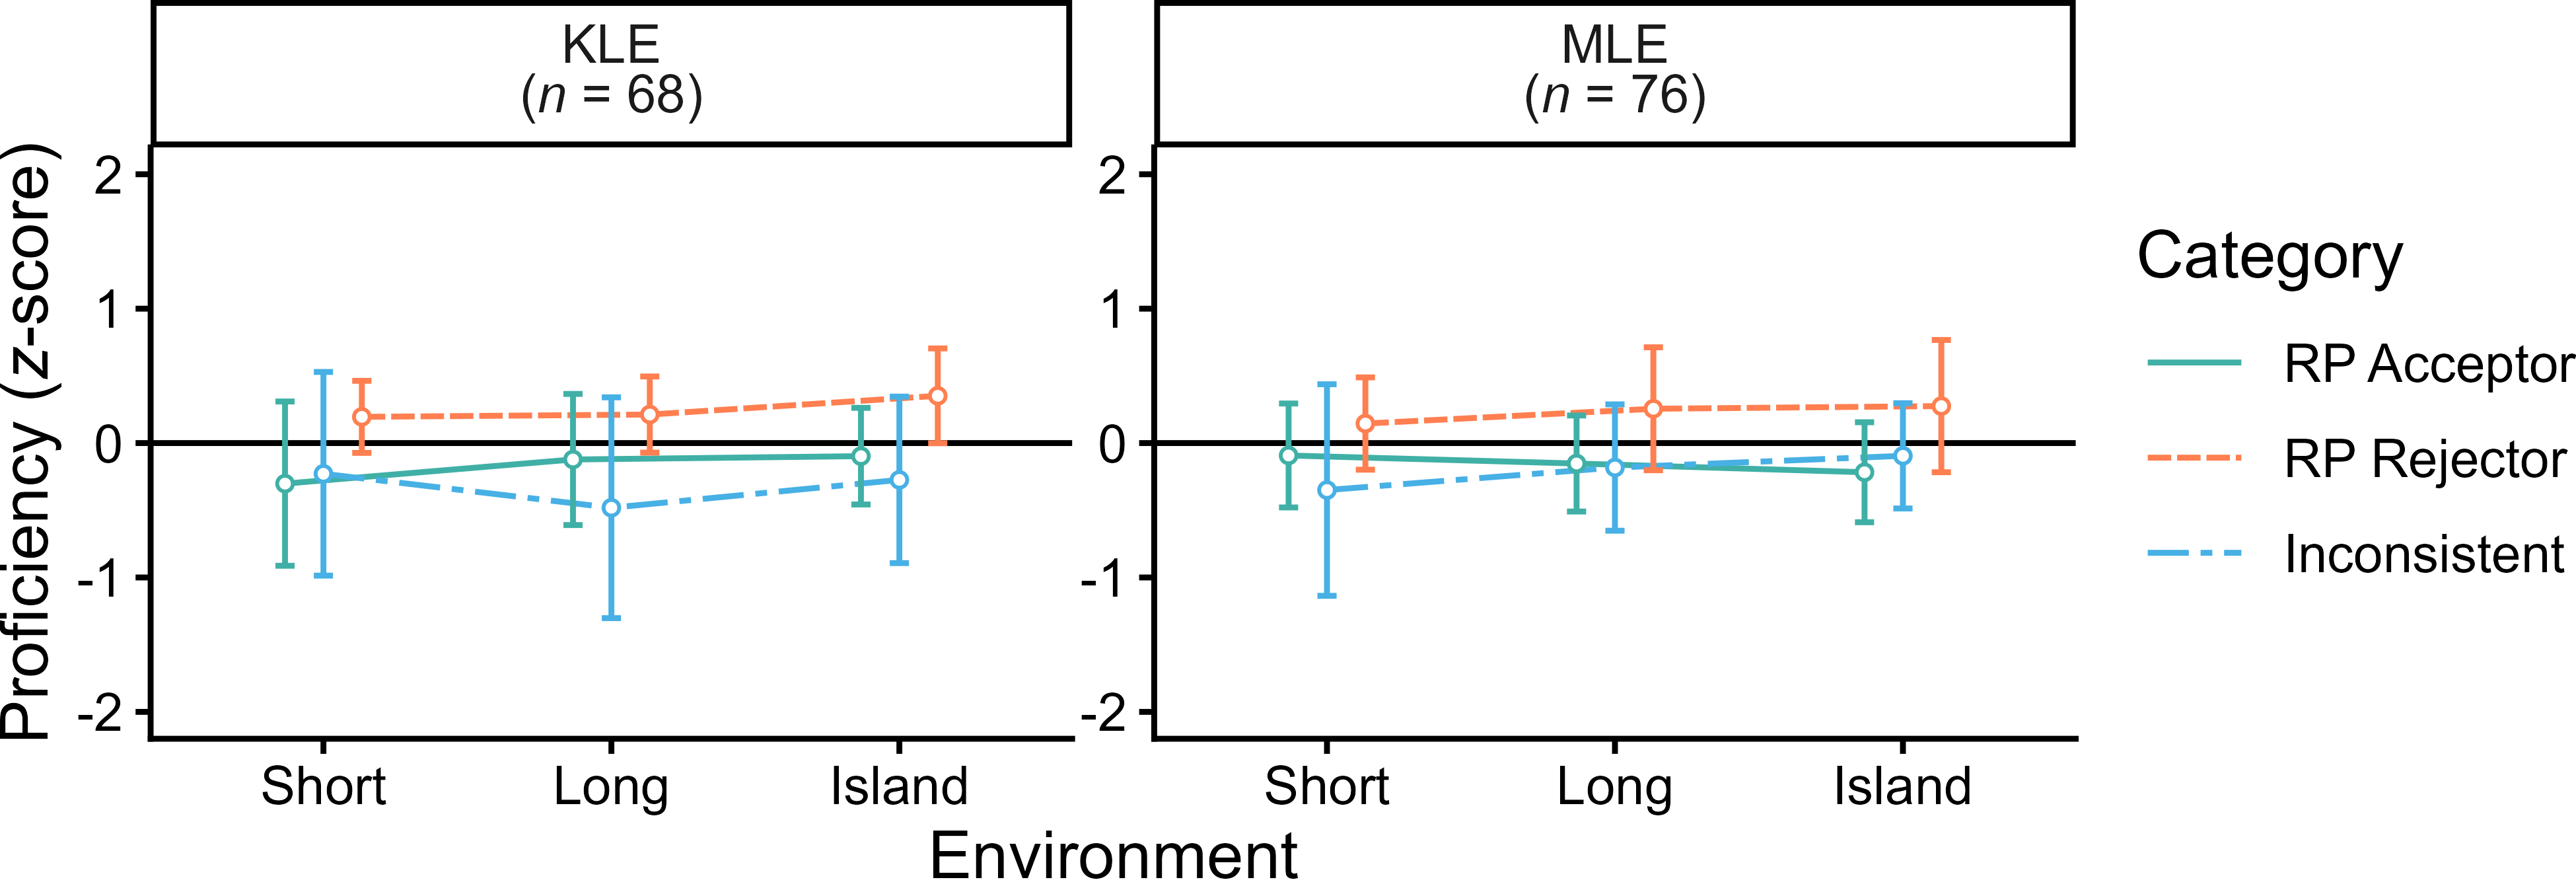
\includegraphics[width=\textwidth]{../analysis/plots/orc_ajt_acceptor_environment_proficiency2.png}
\vspace{-24pt}
\end{figure}

\begin{figure}
\caption{L2 proficiency scores for RP acceptors, RP rejectors, and inconsistent raters in the SRC English acceptability judgment task} \label{fig:ajt-acceptor-proficiency-src}
\raggedright\setstretch{1}
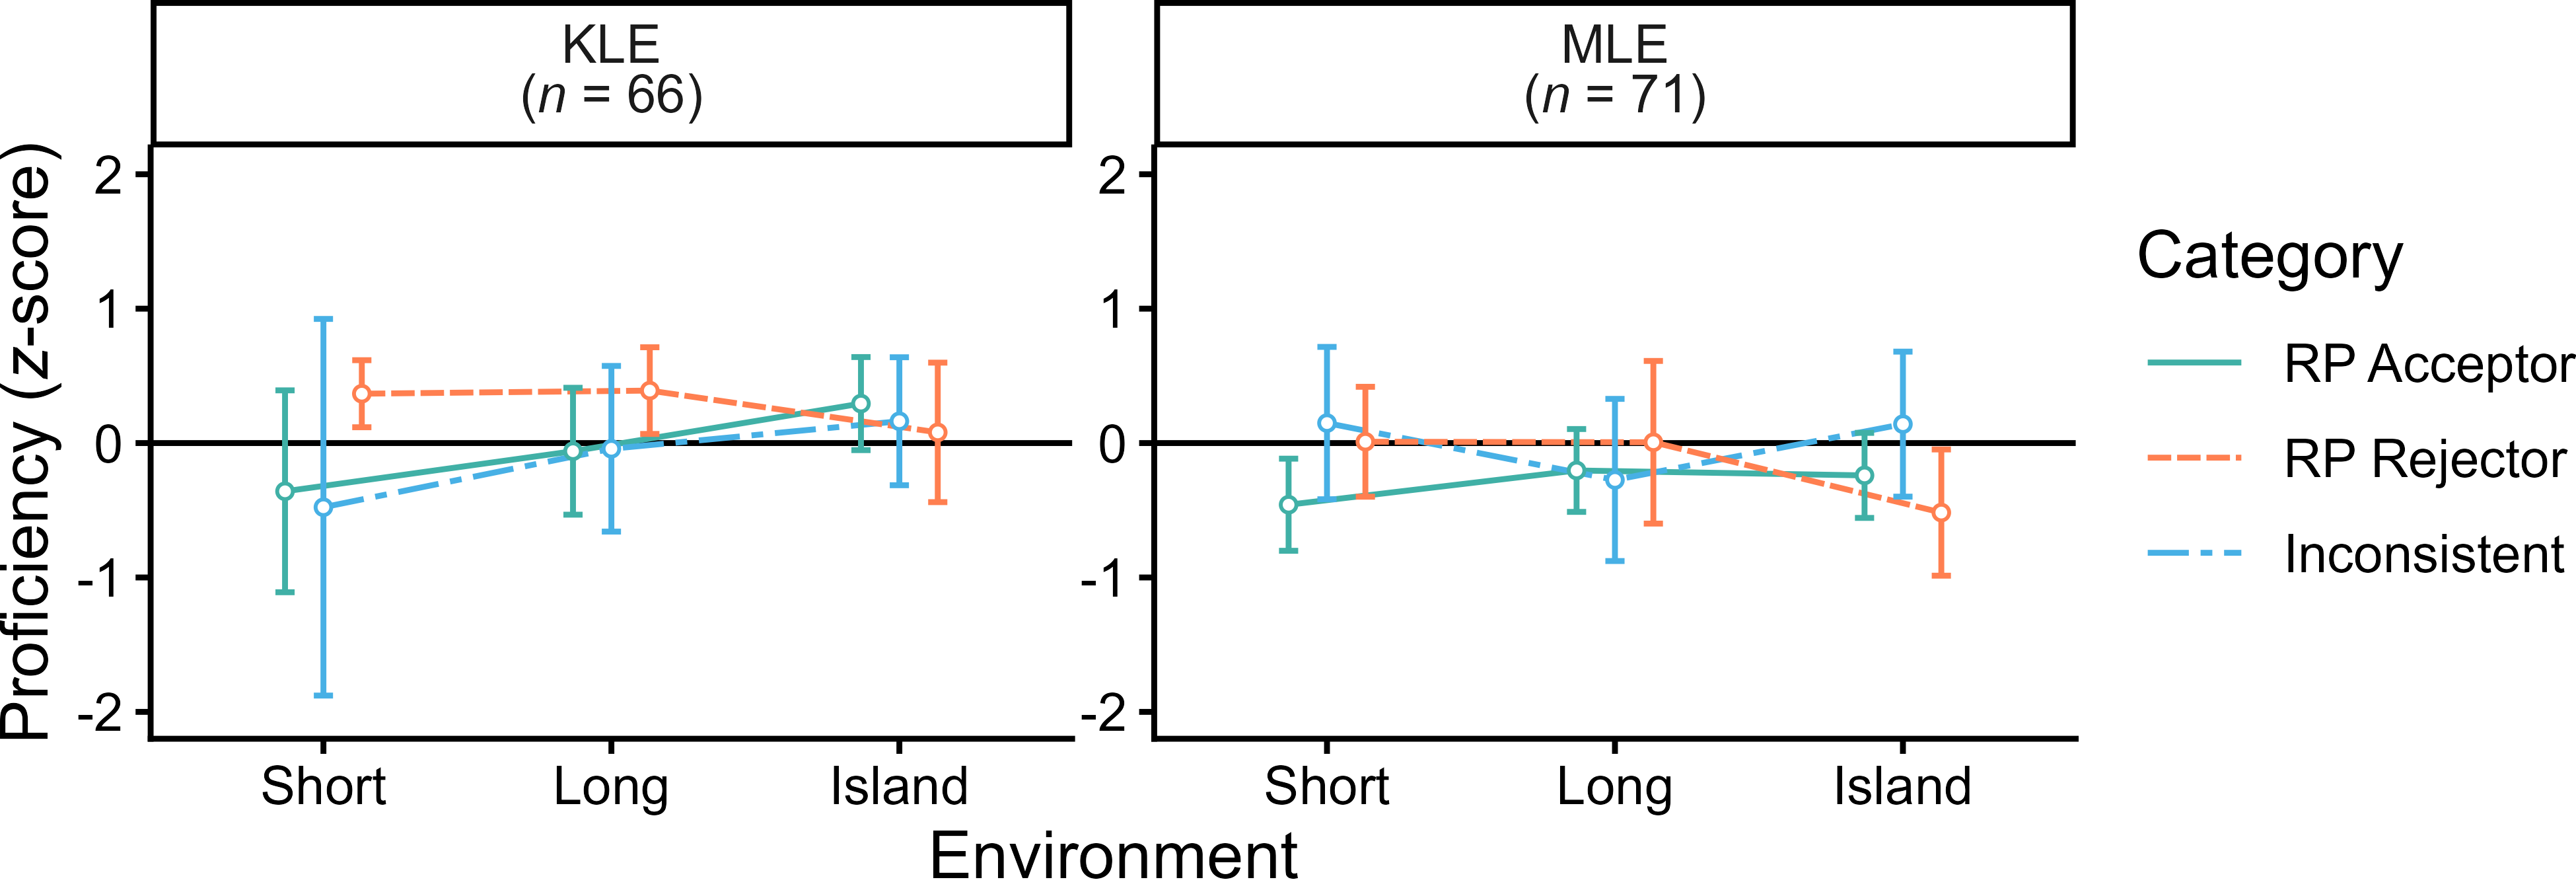
\includegraphics[width=\textwidth]{../analysis/plots/src_ajt_acceptor_environment_proficiency2.png}
\vspace{-24pt}
\end{figure}

\noindent Although the differences in proficiency scores among the RP acceptors, RP rejectors, and inconsistent raters are relatively small in scale, one pattern we can readily identify in the figures is that there was a tendency for RP rejectors to have higher mean proficiency scores. In fact, this pattern holds true across all \textsc{environment} × \textsc{pairing} combinations in the ORC dataset. The SRC dataset presents a somewhat more complex picture, but RP rejectors still had higher mean proficiency scores than at least RP acceptors in the Short and Long conditions. That the SRC Island condition would be the one condition where the pattern breaks down makes sense because, as mentioned earlier in this chapter, there is evidence that in English, \textit{wh}-island SRCs are both (a)~stronger islands than \textit{wh}-island ORCs and (b)~harder to process than \textit{wh}-island ORCs.

To further inspect how L2 proficiency influenced participants' rating patterns, I~refit the ORC and SRC models for the binary [\textsc{±acceptor}] data in the KE and ME pairings with \textsc{proficiency} added as a continuous fixed effect. 

The ORC model (model formula: \textsc{acceptor \~{} environment * pairing * proficiency + (1 | participant)}---see Appendix~\ref{app-results-ajt}, Table~\ref{tblr:app-orc-ajt-acceptor-model} for details) turned up a significant effect of \textsc{proficiency} ($\hat{\beta}$~=~−0.75, \textit{SE}~=~0.36, $p$~=~.036). None of the interactions involving \textsc{proficiency} approached significance (all $p$s~>~.10), though, suggesting that the proficiency effect did not vary to a statistically meaningful degree across levels of \textsc{environment} and \textsc{pairing}.

The SRC model (model formula: \textsc{acceptor \~{} environment * pairing * proficiency + (1 | participant)}---see Appendix~\ref{app-results-ajt}, Table~\ref{tblr:app-src-ajt-acceptor-model} for details) likewise found a significant effect for \textsc{proficiency} ($\hat{\beta}$~=~−0.39, \textit{SE}~=~0.20, $p$~=~.046). However, this time one of the two-way \textsc{environment} × \textsc{proficiency} interactions did rise to the level of significance ($p$~=~.008). Pairwise comparisons revealed that the proficiency effect reached significance for both L2 groups, but only in the Short condition (KLE: $\hat{\beta}$~=~−0.95, \textit{SE}~=~0.47, $p$~=~.044; MLE: $\hat{\beta}$~=~−0.81, \textit{SE}~=~0.37, $p$~=~.029).

These results broadly show that RP acceptance by L2ers is associated with lower English proficiency. As proficiency rises, then, one can expect that participants who initially accept resumptive RCs will eventually start rejecting them. On the individual level, if we can take consistent RP acceptance as evidence that resumption is a permissible option for relativization in a participant's interlanguage grammar, then these results indicate both (a)~that at least some KLEs and MLEs have grammatical resumption in their interlanguage English and (b)~that they are able to purge resumption from their interlanguage English as proficiency climbs. There were also signs that the proficiency effect is stronger in the Short condition than in the Long and Island conditions, suggesting that sensitivity to the illicit nature of RPs in English starts in those RC environments where processing is easiest, and eventually extends to other RC environments where processing is more difficult.

%========================================================%
\section{L1 transfer effects}\label{ajt-transfer}
%========================================================%

Finally, we turn to RQ3, which asks whether L2 acceptance of English resumptive RCs can be traced to L1 transfer.
More than half of L2ers in each study consistently accepted RPs for at least one environment in the English AJT: 77 of 144 L2ers (53\%) in the ORC dataset (KLE: 35/68~= 51\%; MLE: 42/76~= 55\%) and 94 of 138 L2ers (68\%) in the SRC dataset (KLE: 36/66~= 55\%; MLE: 58/72~= 81\%). Of the possible reasons why these L2ers might have accepted English RPs, two that we can reasonably hope to identify in the current data are L1 transfer and a \textit{yes} bias. The procedure I~used for categorizing participants was as follows: First, I~flagged RP acceptors as having a potential \textit{yes} bias (henceforth, the `Bias' type) if they accepted ≥ 80\% of both (a)~ungrammatical English AJT fillers and (b)~all English AJT critical trials. Next, I~flagged remaining RP acceptors as potential cases of L1 transfer (henceforth, the `Transfer' type) if they also consistently accepted RPs in at least one of the same environments in their native language. Lastly, I~placed all RP acceptors who had not been sorted into Bias or Transfer types into a third catchall category (henceforth, the `Other' type).

Figures~\ref{fig:ajt-acceptor-type-orc} and \ref{fig:ajt-acceptor-type-src} show the proportion of RP acceptors who were sorted into each of the three categories in, respectively, the ORC data and the SRC data.

\begin{figure}
\caption{Percentage of RP acceptors by type in the English ORC acceptability judgment tasks} \label{fig:ajt-acceptor-type-orc}
\raggedright\setstretch{1}
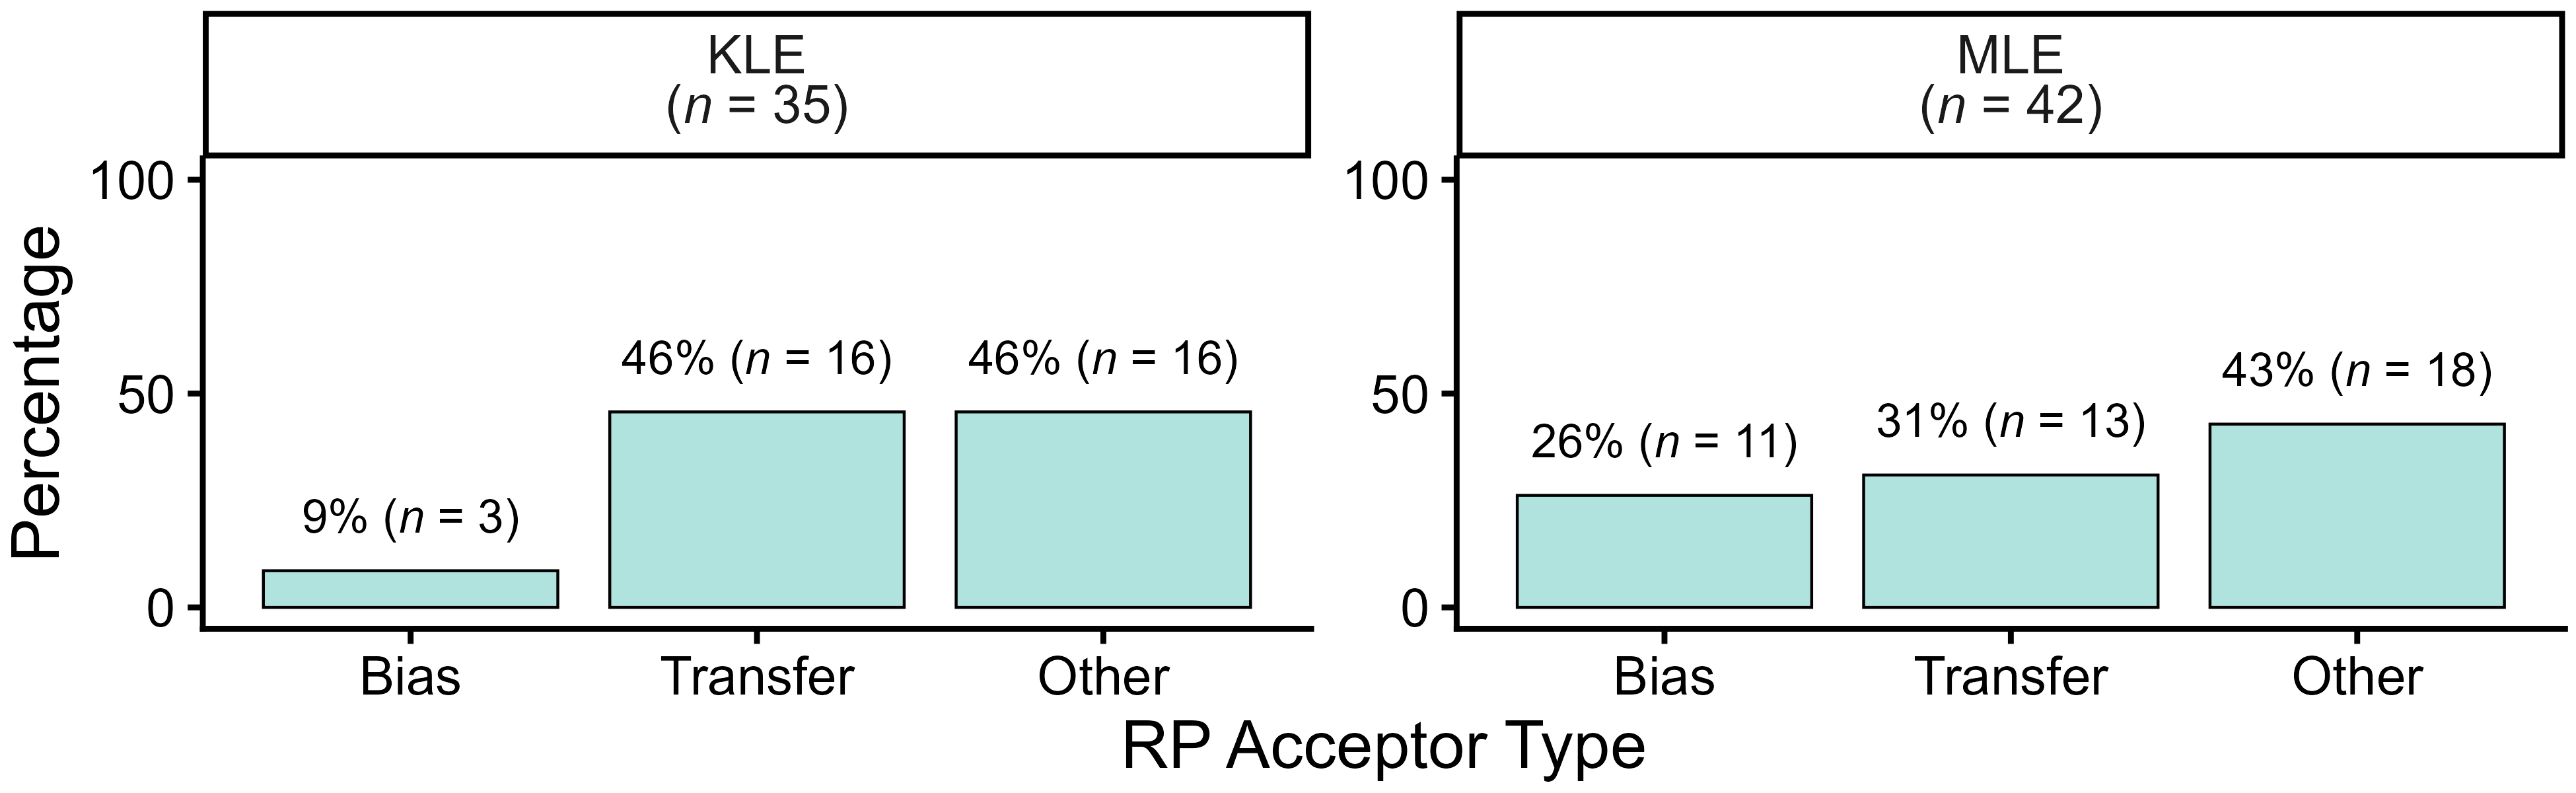
\includegraphics[width=\textwidth]{../analysis/plots/orc_ajt_acceptor_type.png}
\vspace{-24pt}
\end{figure}

\begin{figure}
\caption{Percentage of RP acceptors by type in the English SRC acceptability judgment tasks} \label{fig:ajt-acceptor-type-src}
\raggedright\setstretch{1}
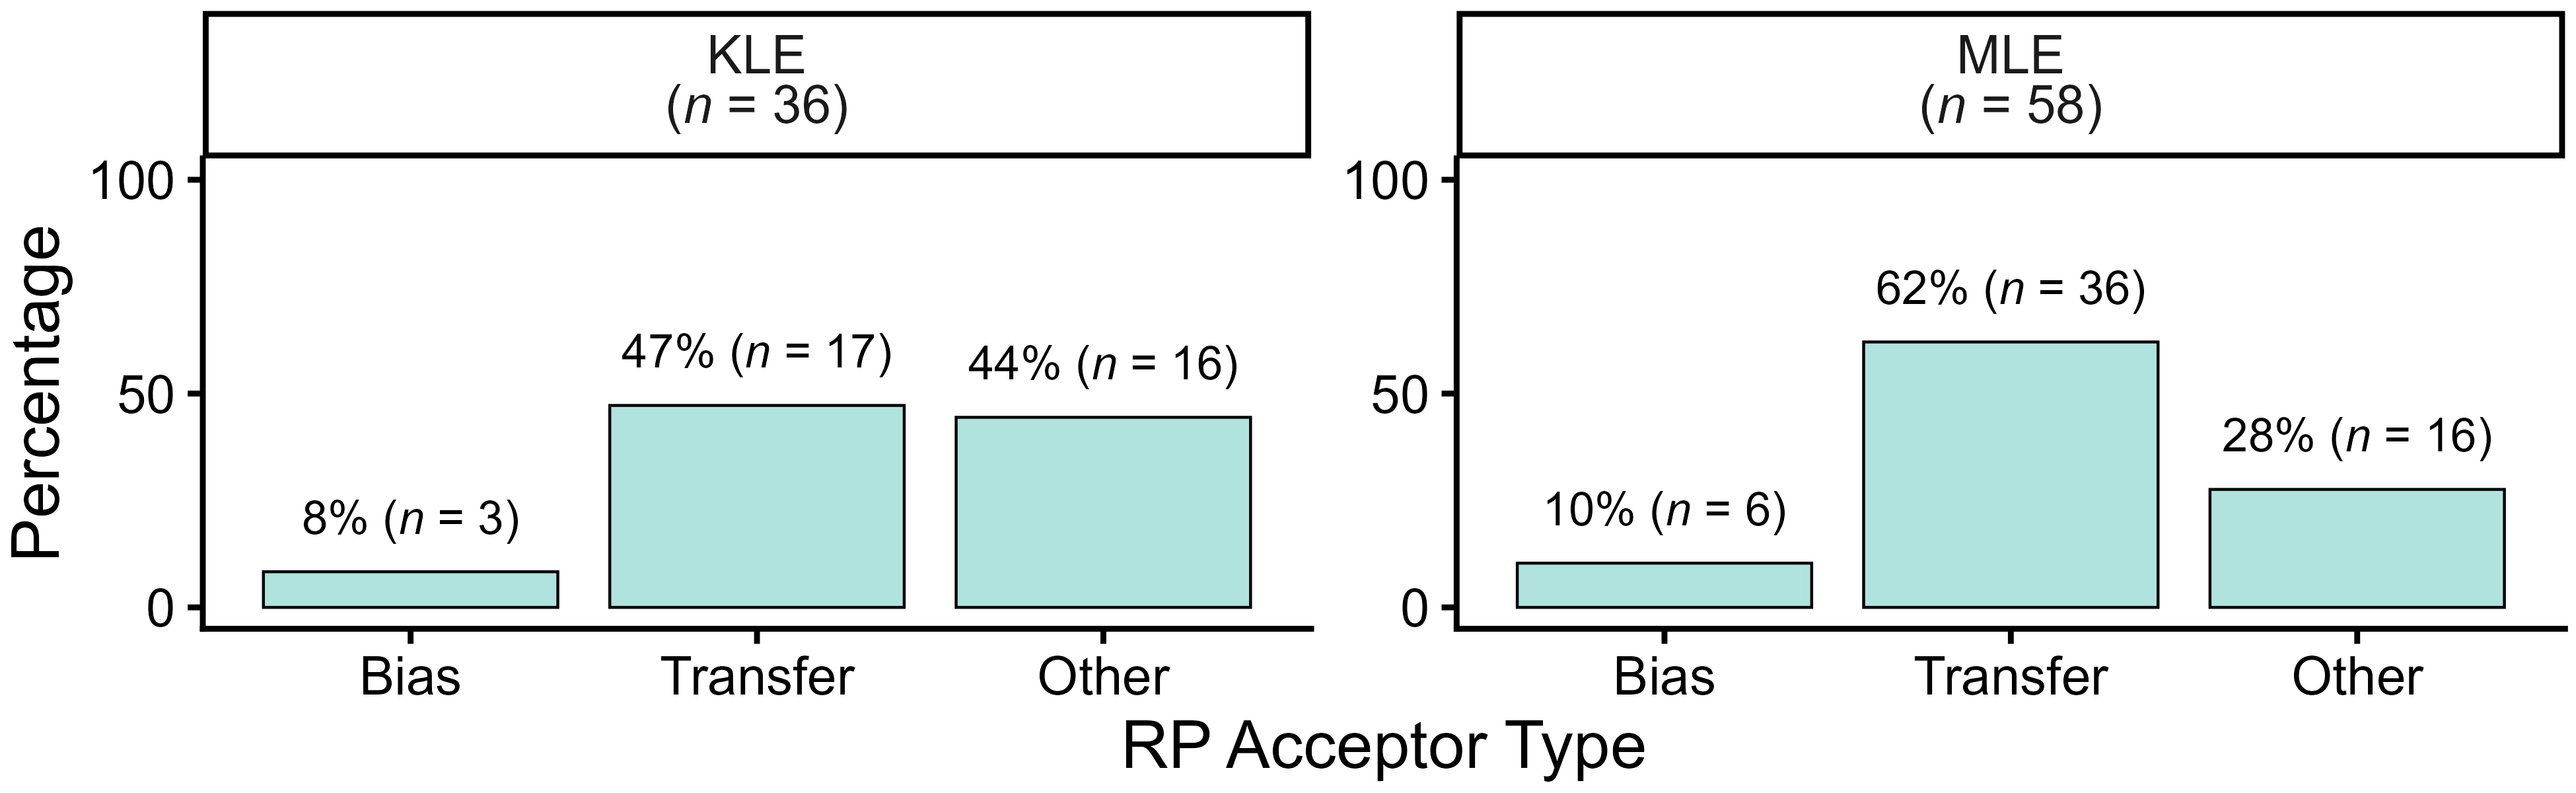
\includegraphics[width=\textwidth]{../analysis/plots/src_ajt_acceptor_type.png}
\vspace{-24pt}
\end{figure}

\noindent Individuals of the Bias type accounted for a relatively small portion of RP-accepting L2ers: 14 of 77  RP-accepting L2ers (18\%) in the ORC dataset (KLE: 3/35~= 9\%; MLE: 11/42~= 26\%) and 9 of 94 RP-accepting L2ers (10\%) in the SRC dataset (KLE: 3/36~= 8\%; MLE: 6/58~= 10\%). The low incidence of Bias participants was expected since the rating data had already undergone a round of cleaning in which participants with strong \textit{yes} or \textit{no} biases were identified and removed (see~Section~\ref{ajt-analysis}). As predicted, L2 acceptance of English resumptive RCs could be traced much of the time to possible L1 transfer, with participants in the Transfer group amounting to 29 of 77 RP-accepting L2ers (38\%) in the ORC dataset (KLE: 16/35~= 46\%; MLE: 13/42~= 31\%) and 53 of 94 RP-accepting L2ers (56\%) in the SRC dataset (KLE: 17/36~= 47\%; MLE: 36/58~= 62\%). Finally, there was a fairly large proportion of RP-accepting L2ers who could not be accounted for tidily in terms of either L1 transfer or \textit{yes}~bias: 34 of 77 (44\%) in the ORC dataset (KLE: 16/35~= 46\%; MLE: 18/42~= 43\%) and 32 of 94 (34\%) in the SRC dataset (KLE: 16/36~= 44\%; MLE: 16/58~= 28\%). These Other participants formed a non-negligible minority of all the L2ers tested, working out to about a quarter of the total number of L2ers in each study (ORC: 34/144~= 24\%; SRC: 32/138~= 23\%).

%========================================================%
\section{Summing up}\label{ajt-conclusion}
%========================================================%

In the English AJT, ENSs performed much the same as participants in other studies on L1 English resumption: Their ratings for gaps were high in the Short and Long conditions but not the Island condition, and their ratings for RPs were low across all conditions. These results indicate that RPs do not represent a licit option for RC formation in L1 English. 

The results for KLEs and MLEs were more of a mixed bag. While some performed like ENSs in each condition, there were also quite a few who consistently accepted RPs in one or more conditions in the English AJT. For many of these L2ers, their acceptance of RPs could be plausibly traced to either L1 transfer or a general \textit{yes} bias. However, a fair number of L2ers---roughly a quarter of all the L2ers---fell into the Other category because their RP acceptance could not be straightforwardly attributed to either L1 transfer or \textit{yes} bias. This outcome suggests that there may be another avenue besides L1 transfer and target language input by which resumptive RCs can come to be perceived as acceptable in interlanguages.

Another major finding that emerged from the L2 data analyses is that higher English proficiency was associated both with higher ratings for gaps and with lower ratings for RPs, at least in environments where gaps are permitted in English. This suggests that regardless of what the initial state of the interlanguage grammar might look like, L2ers are able to become sensitive to the fact that English allows gapped but not resumptive RCs. The proficiency effect was strongest at the top of the SLW hierarchy, indicating that this sensitivity develops fastest in environments where processing is relatively easy.

The results from the Korean and Mandarin AJTs sometimes deviated from my expectations. The most striking of these had to do with ratings for RPs: Rates of RP acceptance were higher than expected in Korean and lower than expected in Mandarin. This pattern of results is at odds with much of the existing literature on those languages, it being widely affirmed that Mandarin has grammatical resumption in most of the environments I~tested (\cite{keenan.comrie1977}, p.~93; \cite{li.wei2014}, p.~286; \cite{pan2016}, p.~292ff) whereas Korean does not (\cite{keenan.comrie1977}, p.~93; \cite{han2013}, p.~339). This disparity between claims made in the literature and the findings of the current experiment highlights the need for more experimental work probing resumption in Korean and Mandarin. I~return to this topic in Section~\ref{dis-kozh}, where I~explore possible reasons for these unexpected rating patterns in the Korean and Mandarin AJTs.

We have now covered the results from each of the main tasks in the dissertation. In the next chapter, I~reanalyze the EPT data and the SPRT data with RP acceptors removed in order to investigate whether it was the RP acceptors who were the drivers of the processing effects observed in those two tasks.